This appendix presents more details on the measurement of the data-driven real lepton efficiency using the $Z$ tag-and-probe method.

%%%
%%%
%%%

\section{The $Z$ tag-and-probe method}
\label{sec:app_RLE_ZTandP_method}
The $Z$ tag-and-probe method is used to extract the leptons from data and measure the real lepton efficiency.
The selected events are required to have at least two baseline leptons.
The lepton candidates with $\pt > 25$~{\GeV} and satisfying all the signal lepton requirements are categorized into \textit{tag leptons}.
The lepton candidates passing baseline lepton requirements can be classified as \textit{probe leptons}.
In order to form a tag-and-probe pair, the two selected leptons have to carry the same flavor and opposite charge.
The invariant mass of the tag-and-probe pair system should satisfy the $Z$ boson mass window $80 < m_{\ell \ell} < 100$~{\GeV}.
All possible combinations of the tag-and-probe pairs are considered to avoid any bias and to increase the statistics.
For the $Z \to ee$ decay, an additional $|\eta| < 2$ requirement is applied on the tag and probe leptons.
However, no additional requirement is applied for the $Z \to \mu \mu$ decay.
The tag lepton is used to select the probe lepton only and the probe lepton is used for the real efficiency measurements.
In this study, the tag and probe leptons are required to match the lepton triggers listed in Table~\ref{tab:app_RLE_single_lepton_triggers}.

\begin{table}[htbp]
    %\begin{center}
    \resizebox{\textwidth}{!}{% <------ Don't forget this %
        \begin{tabular}{cccc}
            \hline
            \hline
            Trigger                                & lepton   & 2015                                     & 2016\\
            \hline
            \multirow{2}{*}{Single lepton trigger} & electron & \texttt{e24\_lhmedium\_iloose\_L1EM20VH} & \texttt{e26\_lhtight\_nod0\_ivarloose}\\
                                                   & muon     & \texttt{mu20\_iloose\_L1MU15}            & \texttt{mu26\_ivarmedium}\\
            \hline
            \multirow{2}{*}{Dilepton trigger}      & electron & \texttt{2e12\_lhloose\_L12EM10VH}        & \texttt{2e17\_lhvloose\_nod0}\\
                                                   & muon     & \texttt{mu18\_mu8noL1}                   & \texttt{mu22\_mu8noL1}\\
            \hline
            \hline
        \end{tabular}
    }
    %\end{center}
    \caption{The list of single lepton and dilepton triggers used for the real lepton efficiency measurements.
    The dilepton triggers are used for studying the systematic uncertainties causing by the trigger.}
    \label{tab:app_RLE_single_lepton_triggers}
\end{table}

Figure~\ref{fig:app_RLE_mll_distributions} shows the data-to-MC comparison of the tag-and-probe pair invariant mass distributions which indicate the need of subtracting the background especially for the probe electron with $\pt < 20$~{\GeV}.
%
\begin{figure}[htbp]
    \begin{center}
        \begin{subfigure}[b]{0.48\textwidth}
            \begin{center}
                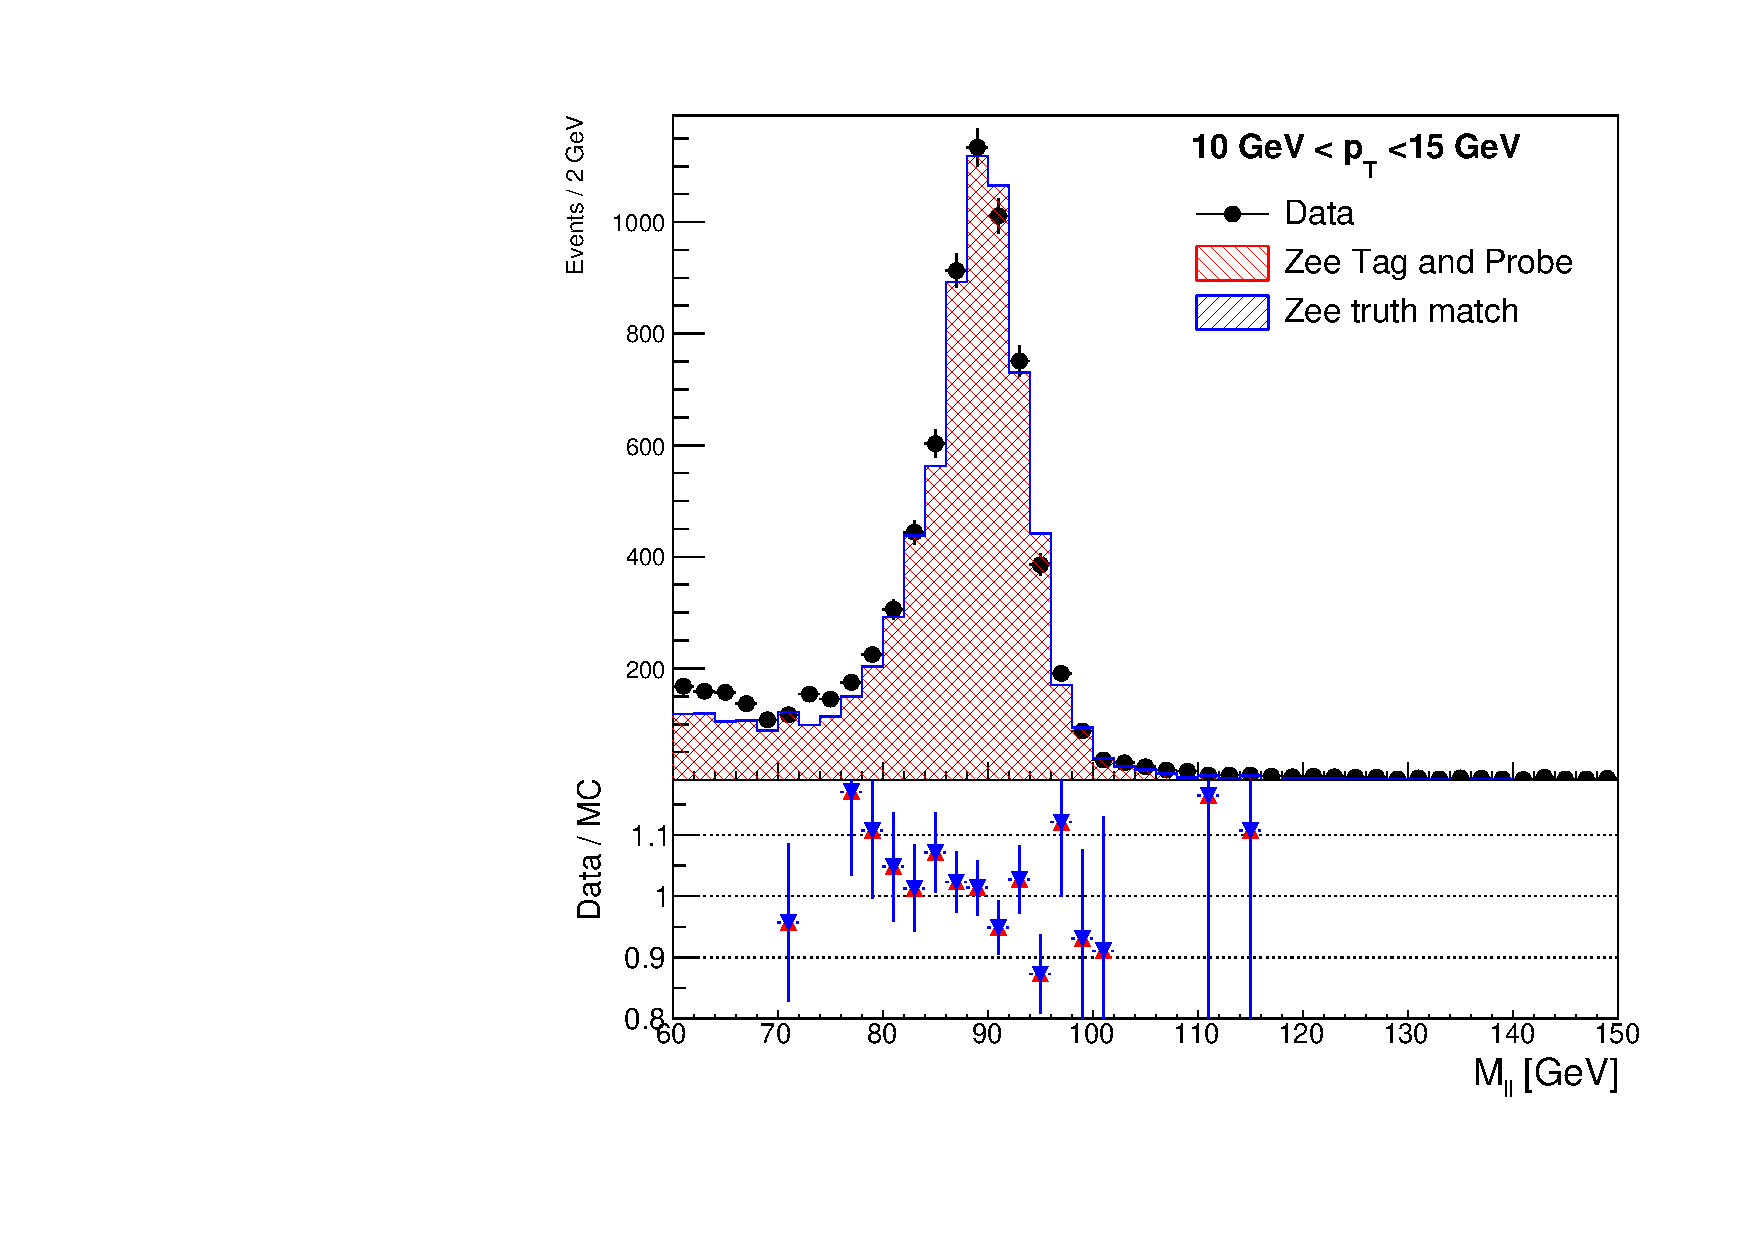
\includegraphics[scale=0.4]{signal_level_Mee_pt1015_ratio_plot_MC_normalized.pdf}
                \caption{The $m_{ee}$ distribution with $10 < \pt < 15$~{\GeV}.}
            \end{center}
        \end{subfigure}%
        \begin{subfigure}[b]{0.48\textwidth}
            \begin{center}
                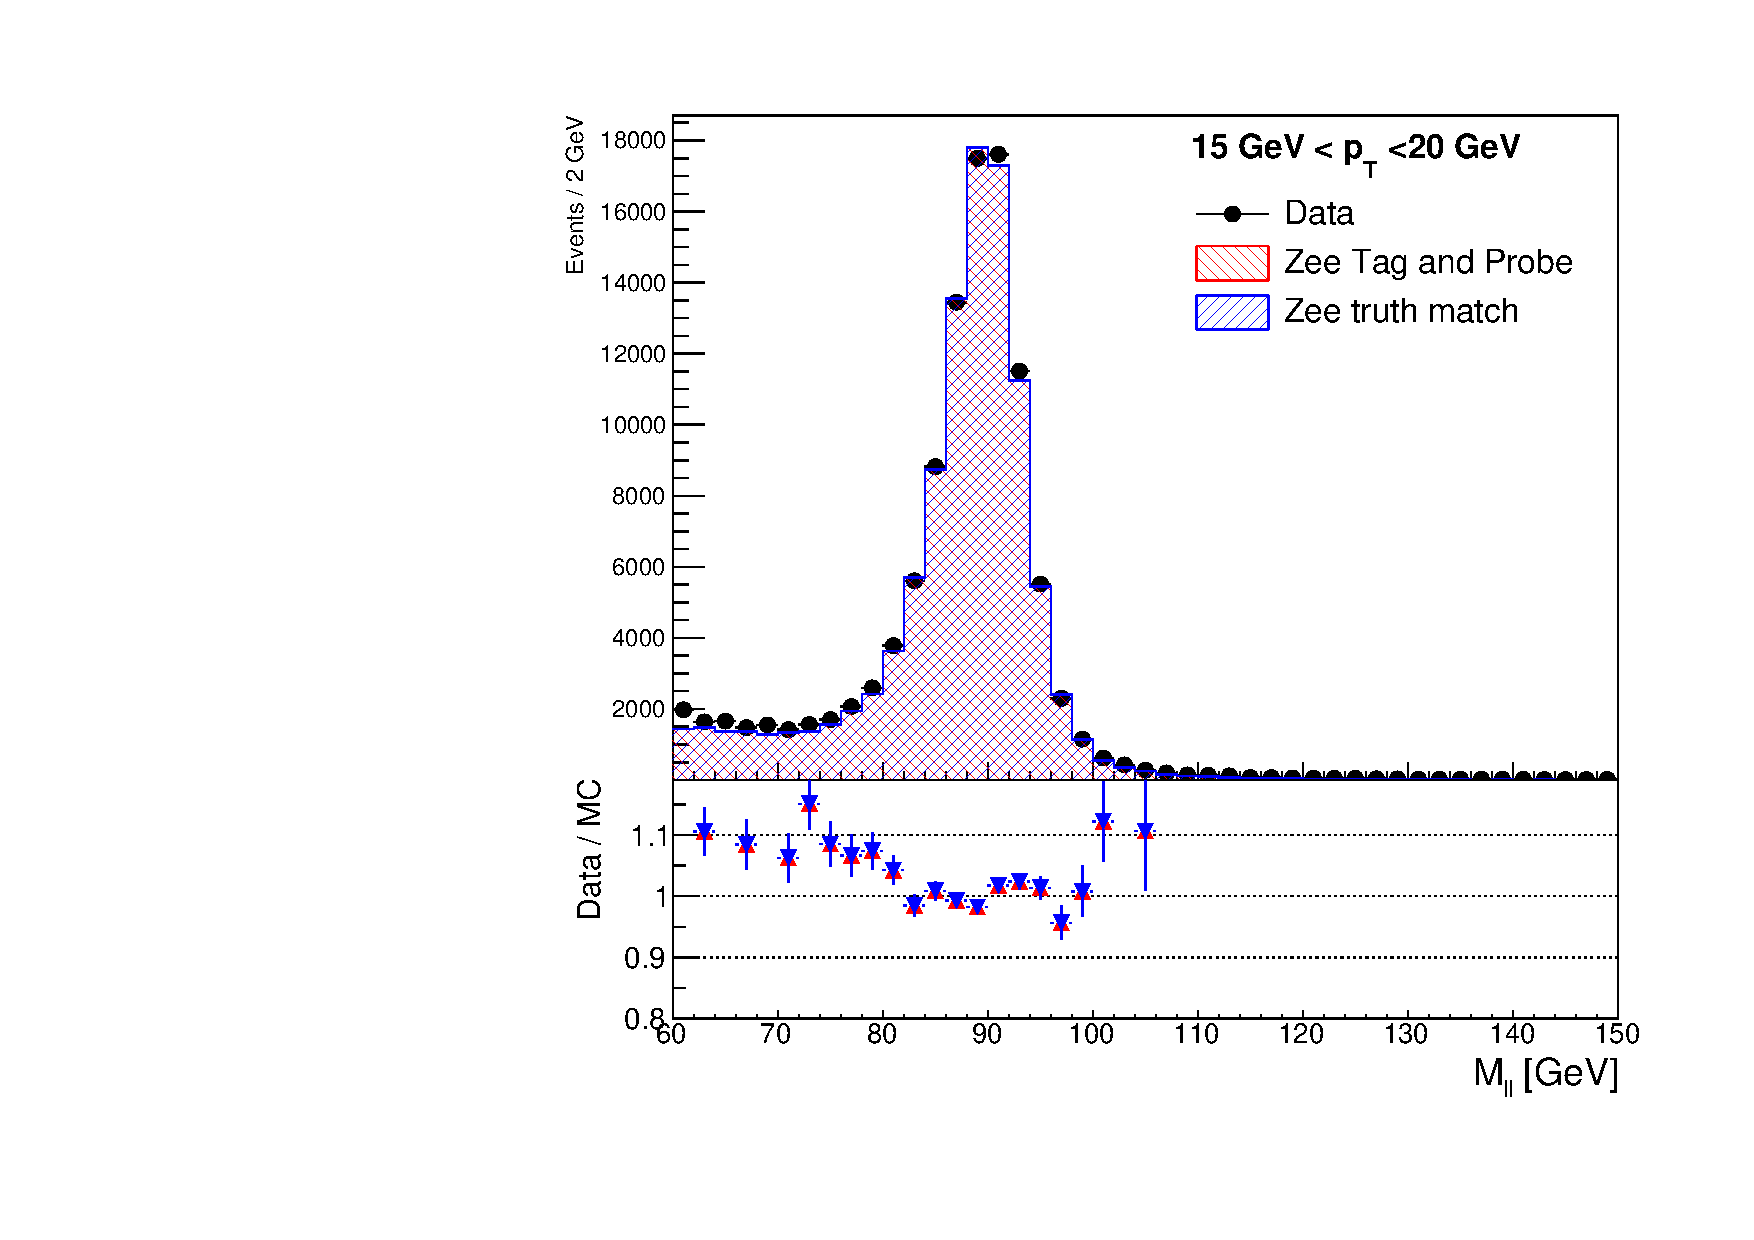
\includegraphics[scale=0.4]{signal_level_Mee_pt1520_ratio_plot_MC_normalized.pdf}
                \caption{The $m_{ee}$ distribution with $15 < \pt < 20$~{\GeV}.}
            \end{center}
        \end{subfigure}
        \begin{subfigure}[b]{0.48\textwidth}
            \begin{center}
                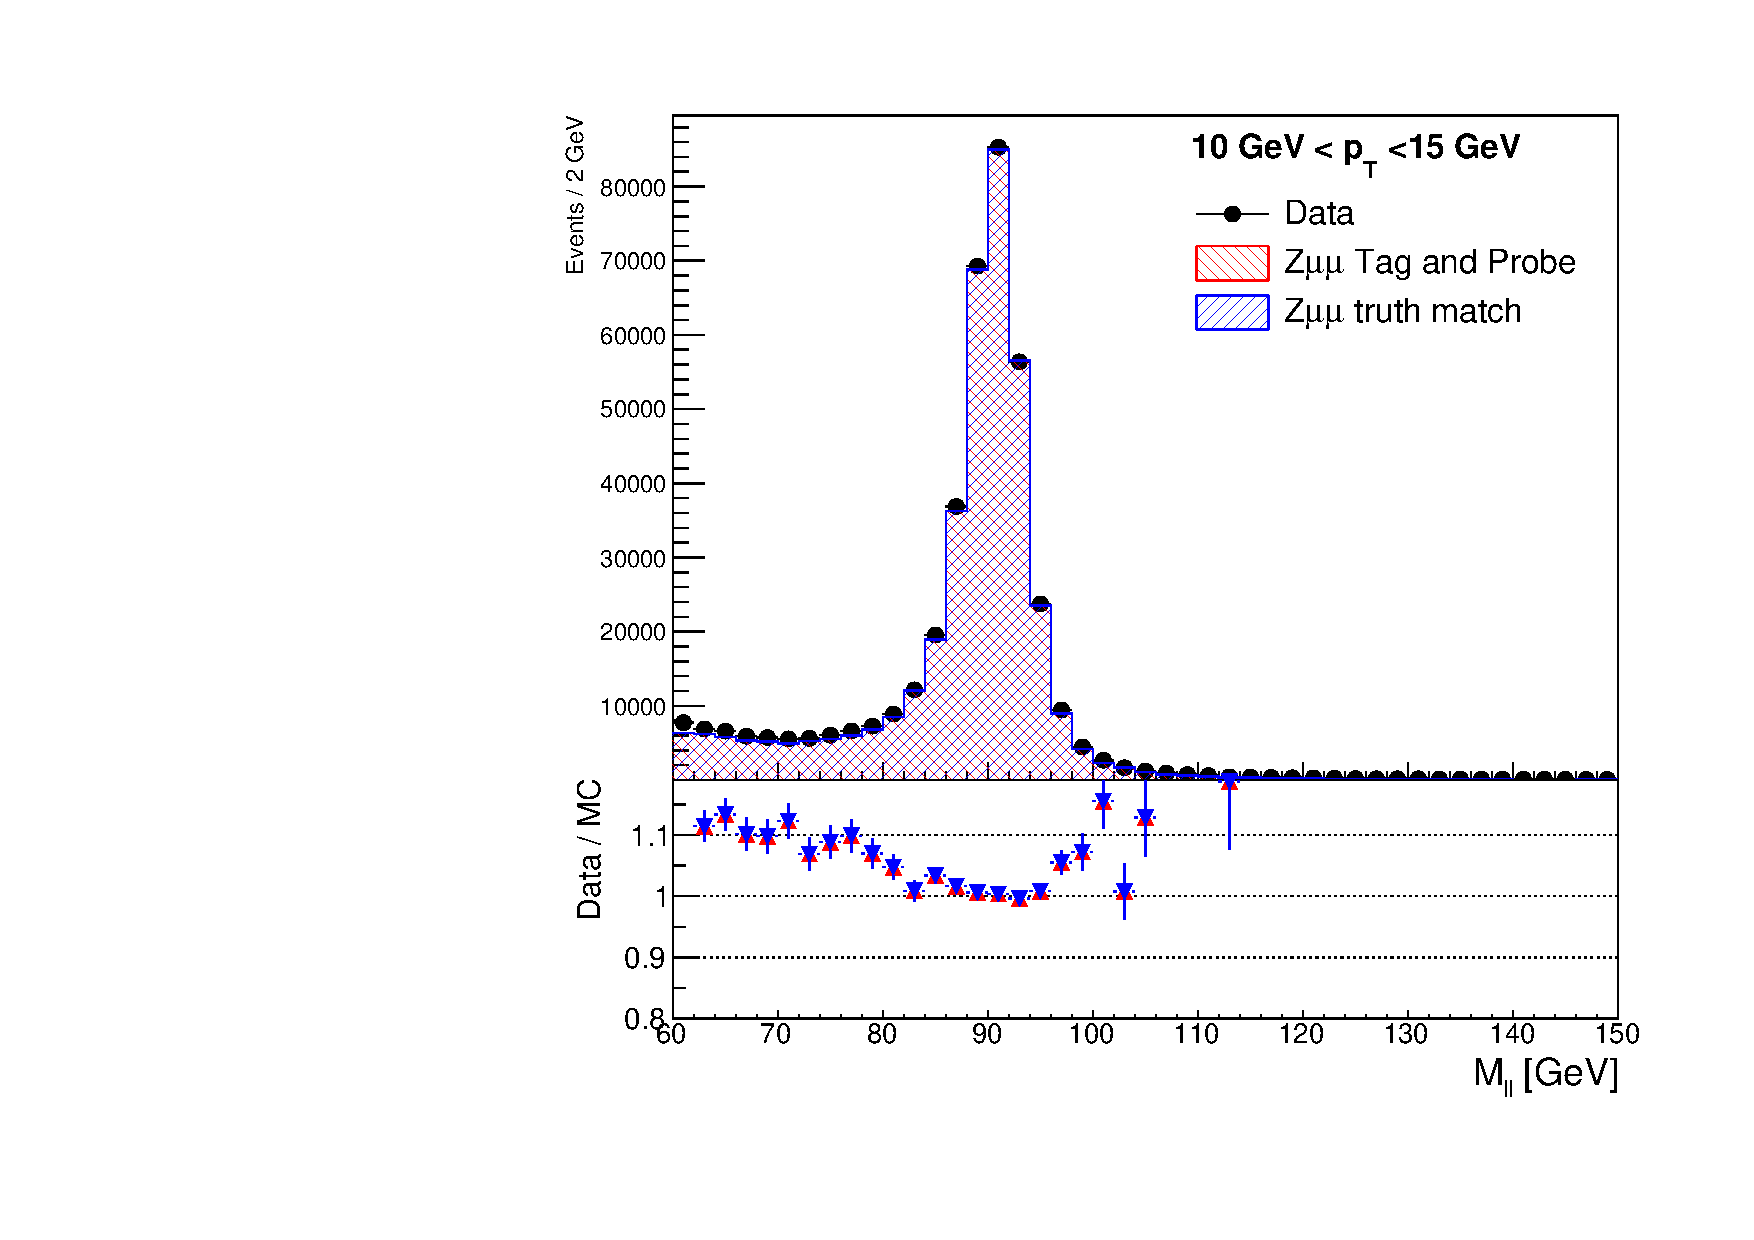
\includegraphics[scale=0.4]{signal_level_Mmumu_pt1015_ratio_plot_MC_normalized.pdf}
                \caption{The $m_{\mu\mu}$ distribution with $10 < \pt < 15$~{\GeV}.}
            \end{center}
        \end{subfigure}%
        \begin{subfigure}[b]{0.48\textwidth}
            \begin{center}
                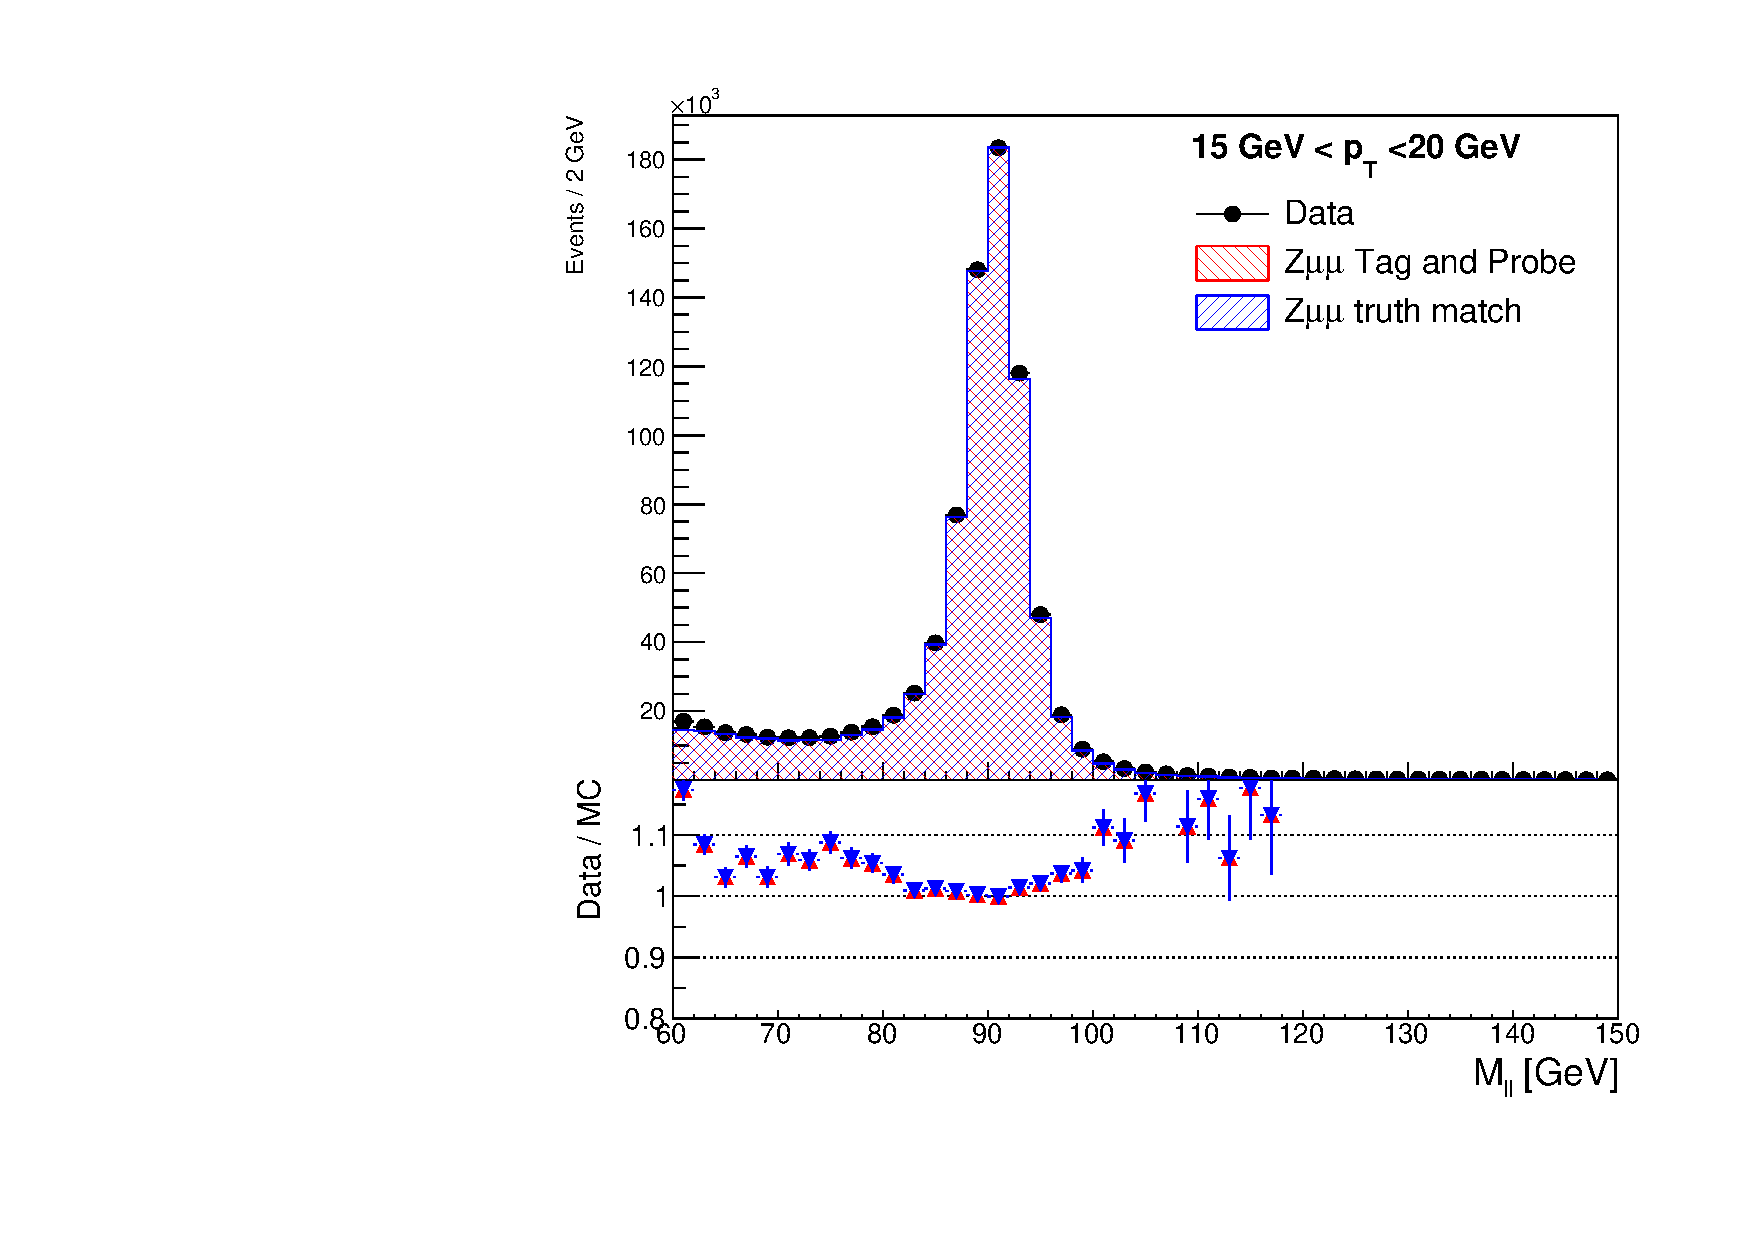
\includegraphics[scale=0.4]{signal_level_Mmumu_pt1520_ratio_plot_MC_normalized.pdf}
                \caption{The $m_{\mu\mu}$ distribution with $15 < \pt < 20$~{\GeV}.}
            \end{center}
        \end{subfigure}
    \end{center}
    \caption{The invariant mass distributions of the tag-and-probe pair computed using $Z+jets$ MC and 2015 + 2016 data.
    The red color stands for the $Z$ tag-and-probe events, the blue color represents the $Z$ truth matched events, and the black dots are data.
    The MC distributions are scaled to the data using a Gaussian fit of the $Z$ mass peak $85 < m_{\ell \ell} < 95$~{\GeV}.}
    \label{fig:app_RLE_mll_distributions}
\end{figure}
%
A background template method, which is similar to the one used by the $e/\gamma$ performance group for their efficiency measurements~\cite{ATLAS-CONF-2014-018}, is used to estimate the background contamination from the low \pt electrons.
No background subtraction is performed on the signal leptons because the background contamination is found to be negligible.
However, the background contamination in the baseline probe leptons needs to be subtracted.
The real lepton efficiency is obtained by the following equation
%
\begin{equation}
    \epsilon = \frac{N_{\mathrm{signal}}}{N_{\mathrm{baseline}} - N_{\mathrm{baseline}}^{bkg}}
    \label{eq:app_RLE_efficiency_formula}
\end{equation}
%
where $N_\mathrm{signal}$ is the number of probe leptons passing the signal requirements, $N_\mathrm{baseline}$ is the number of probe leptons passing the baseline requirements, and $N_\mathrm{baseline}^{bkg}$ is the estimated background contamination in the baseline probe leptons.

%%%
%%%
%%%

\section{Background subtraction}
\label{sec:app_RLE_bkg_subtraction}
The background template method is used to evaluate the background contamination on data.
By inverting the calorimeter and track isolations, requesting the electron object to fail the medium LH identification, the background sample enriched template can be obtained.
Three background templates are considered for the systematic study.
The definitions of the background template are summarized in Table~\ref{tab:app_RLE_bkg_templates}.
%
\begin{table}[htbp]
    %\begin{center}
    \resizebox{\textwidth}{!}{% <------ Don't forget this %
        \begin{tabular}{cccc}
            \hline
            \hline
            cut                   & variation 1 template                   & baseline template                       & variation 2 template\\
            \hline
            Identification        & -                                      & fail medium LH                          & fail medium LH\\
            Calorimeter isolation & $E_\mathrm{T}^{topocone20} /\pt > 6\%$ & $E_\mathrm{T}^{topocone20} /\pt > 15\%$ & $E_\mathrm{T}^{topocone20} /\pt > 20\%$\\
            Track isolation       & $p_\mathrm{T}^{varcone20} /\pt > 6\%$  & $E_\mathrm{T}^{topocone20} /\pt > 8\%$  & $E_\mathrm{T}^{topocone20} /\pt > 15\%$\\
            \hline
            \hline
        \end{tabular}
    }
    %\end{center}
    \caption{The definition of the background templates for estimating the background contamination associated with the $Z$ tag-and-probe method.
    The baseline template is used to estimate the background contamination.
    The variation 1 template has looser requirements and the variation 2 template has tighter requirements.
    They are used to assess the systematic caused by the background contamination.}
    \label{tab:app_RLE_bkg_templates}
\end{table}
%
Figure~\ref{fig:app_RLE_bkg_templates} shows the $m_{ee}$ distributions of the background template.
%
\begin{figure}[htb]
    \begin{subfigure}[b]{0.48\textwidth}
        \begin{center}
            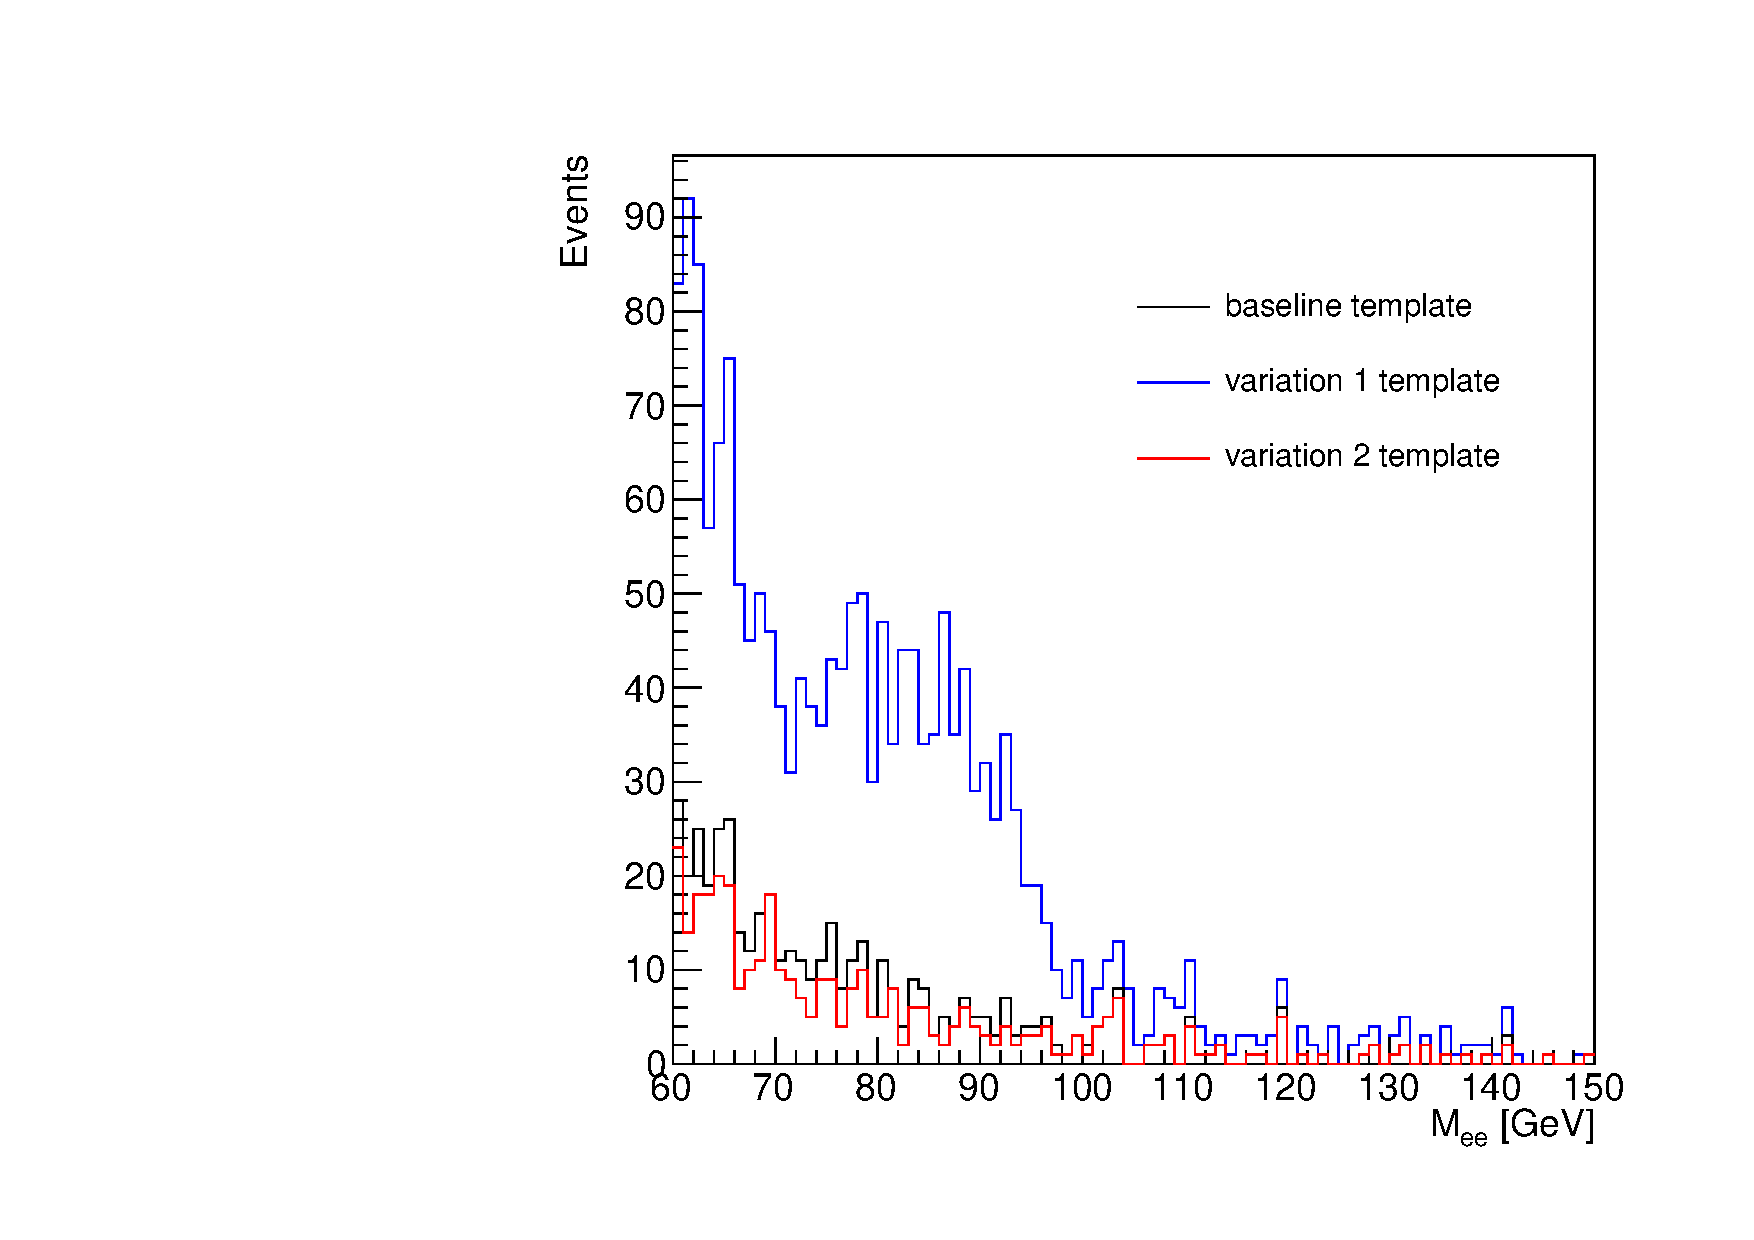
\includegraphics[scale=0.4]{bkg_template_electron_pt_1015_eta0201.pdf}
            \caption{Probe electrons with $10 < \pt < 15$~{\GeV}.}
        \end{center}
    \end{subfigure}
    \begin{subfigure}[b]{0.48\textwidth}
        \begin{center}
            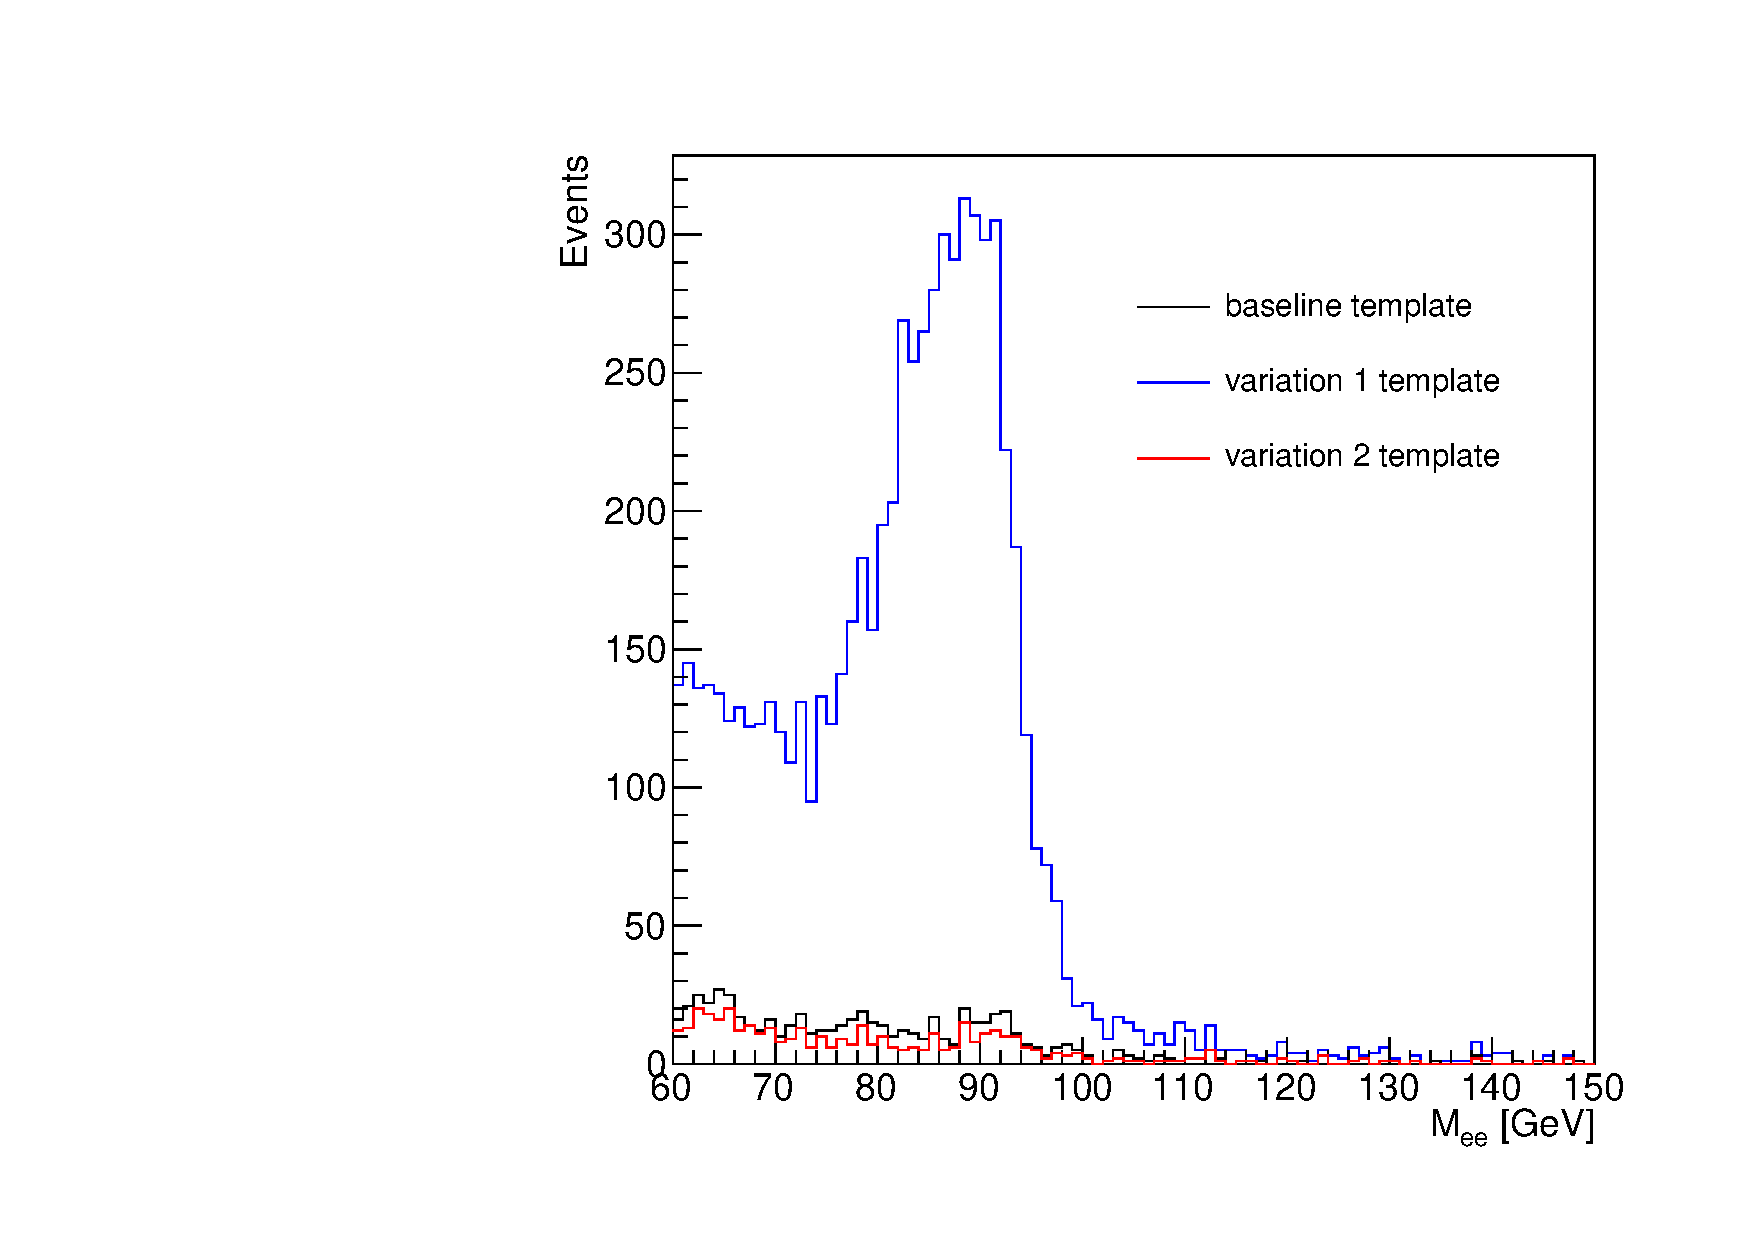
\includegraphics[scale=0.4]{bkg_template_electron_pt_1520_eta0201.pdf}
            \caption{Probe electrons with $15 < \pt < 20$~{\GeV}.}
        \end{center}
    \end{subfigure}
    \caption{The $m_{ee}$ distributions for the baseline, variation 1 and variation 2 background templates.
    The $m_{ee}$ distributions are computed using the probe electrons with different \pt as indicated in the caption of plots.
    The variation 1 template has looser calorimeter and track isolation requirements and the baseline and the variation 2 templates have tighter selection criteria.
    So a peak can be seen in the $Z$ mass region in variation 1 template but not in the baseline and variation 2 templates.}
    \label{fig:app_RLE_bkg_templates}
\end{figure}
%
The invariant mass distribution of the template events ($m_{ee}^\mathrm{template}$) is then used to estimate the amount of background in $80 < m_{\ell \ell} < 100$~{\GeV} region.
In order to estimate the correct of background events, the $120 < m_{ee} < 150$~{\GeV} region is used to normalize the background template because a smaller prompt electron contribution is expected in this region.
Equation~\ref{eq:app_RLE_bkg_in_the_tail} shows the estimation of the number of background events in the tail region using the baseline electrons.
%
\begin{equation}
    N_{bkg}^\mathrm{tail} = N_\mathrm{baseline}^\mathrm{tail} - N_\mathrm{MC, prompt}^\mathrm{tail}
    \label{eq:app_RLE_bkg_in_the_tail}
\end{equation}
%
where $N_\mathrm{baseline}^\mathrm{tail}$ can be obtained by integrating the baseline $m_{ee}$ distribution in the tail region and $N_\mathrm{MC, prompt}^\mathrm{tail}$ is the prompt electron contamination which is estimated by integrating the $m_{ee}$ distribution in the tail region using the $Z \to ee$ MC simulation.
Because the baseline electron selection criteria already provides a relatively high purity of prompt electrons, the background template suffers from low statistics in the tail region.
The template is fitted in region $60 < m_{ee}^\mathrm{template} < 120$~{\GeV} using an exponential function to avoid any bias in the normalization factor due to statistical fluctuations.
However, the $80 < m_{ee}^\mathrm{template} < 100$~{\GeV} is excluded to minimize the prompt lepton contamination arising from $Z \to ee$ decays.
The fit is mostly driven by the $60 < m_{ee}^\mathrm{template} < 80$~{\GeV} due to the low statistics in the tail.
After fitting is performed, the template in the tail region $N_\mathrm{template}^\mathrm{tail}$ is normalized to the background in the tail $N_{bkg}^\mathrm{tail}$ to get the correct estimated number of background events.
The baseline $m_{ee}$ distributions before and after applying the background subtraction using the background template are shown in Fig.~\ref{fig:app_RLE_bkg_estimations}.
%
\begin{figure}[htbp]
    \begin{subfigure}[b]{0.32\textwidth}
        \begin{center}
            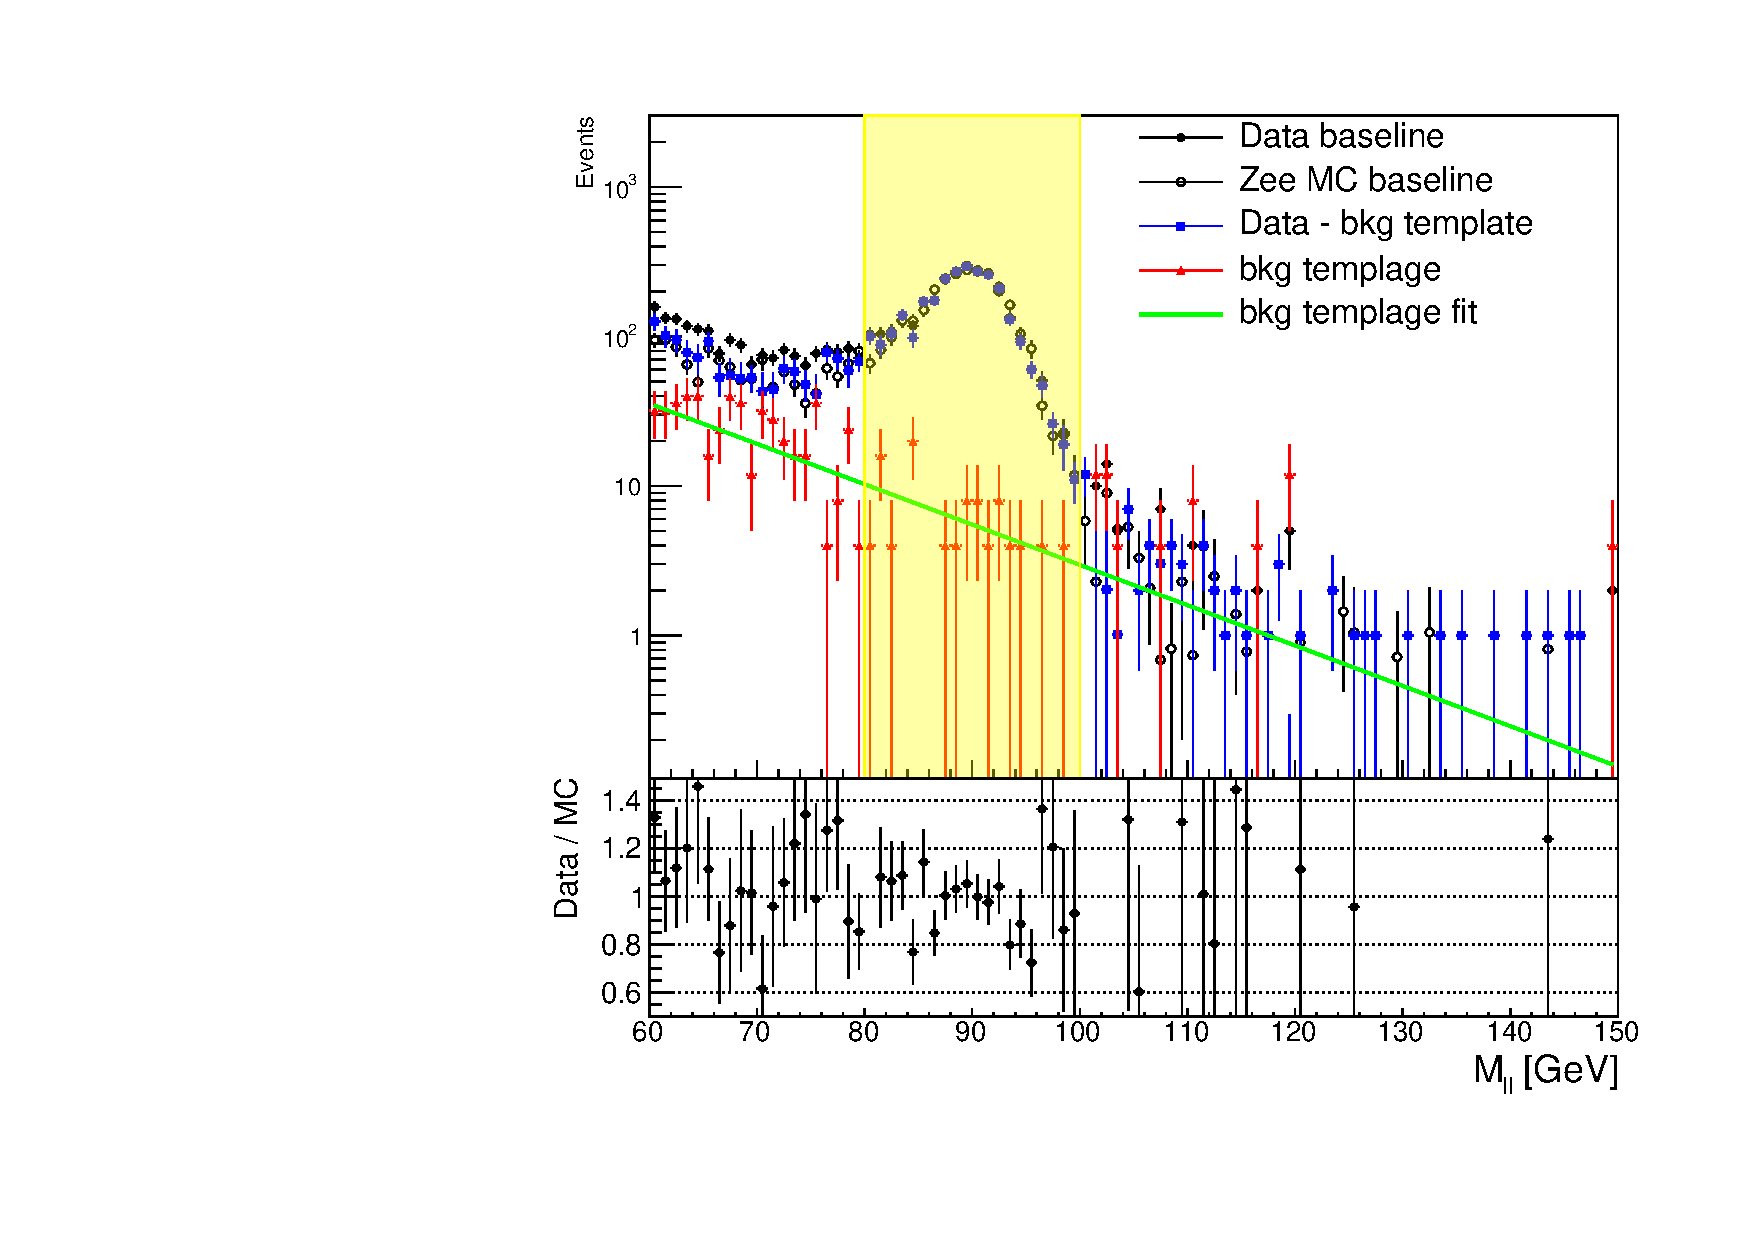
\includegraphics[scale=0.27]{bkg_subtraction_baseline_template_range_baseline_mll80_100_pt10_15_eta0_80_tag_trigger_matched.pdf}
            \caption{$10 < \pt < 15$~{\GeV}\\$0 < |\eta| < 0.8$}
        \end{center}
    \end{subfigure}
    \begin{subfigure}[b]{0.32\textwidth}
        \begin{center}
            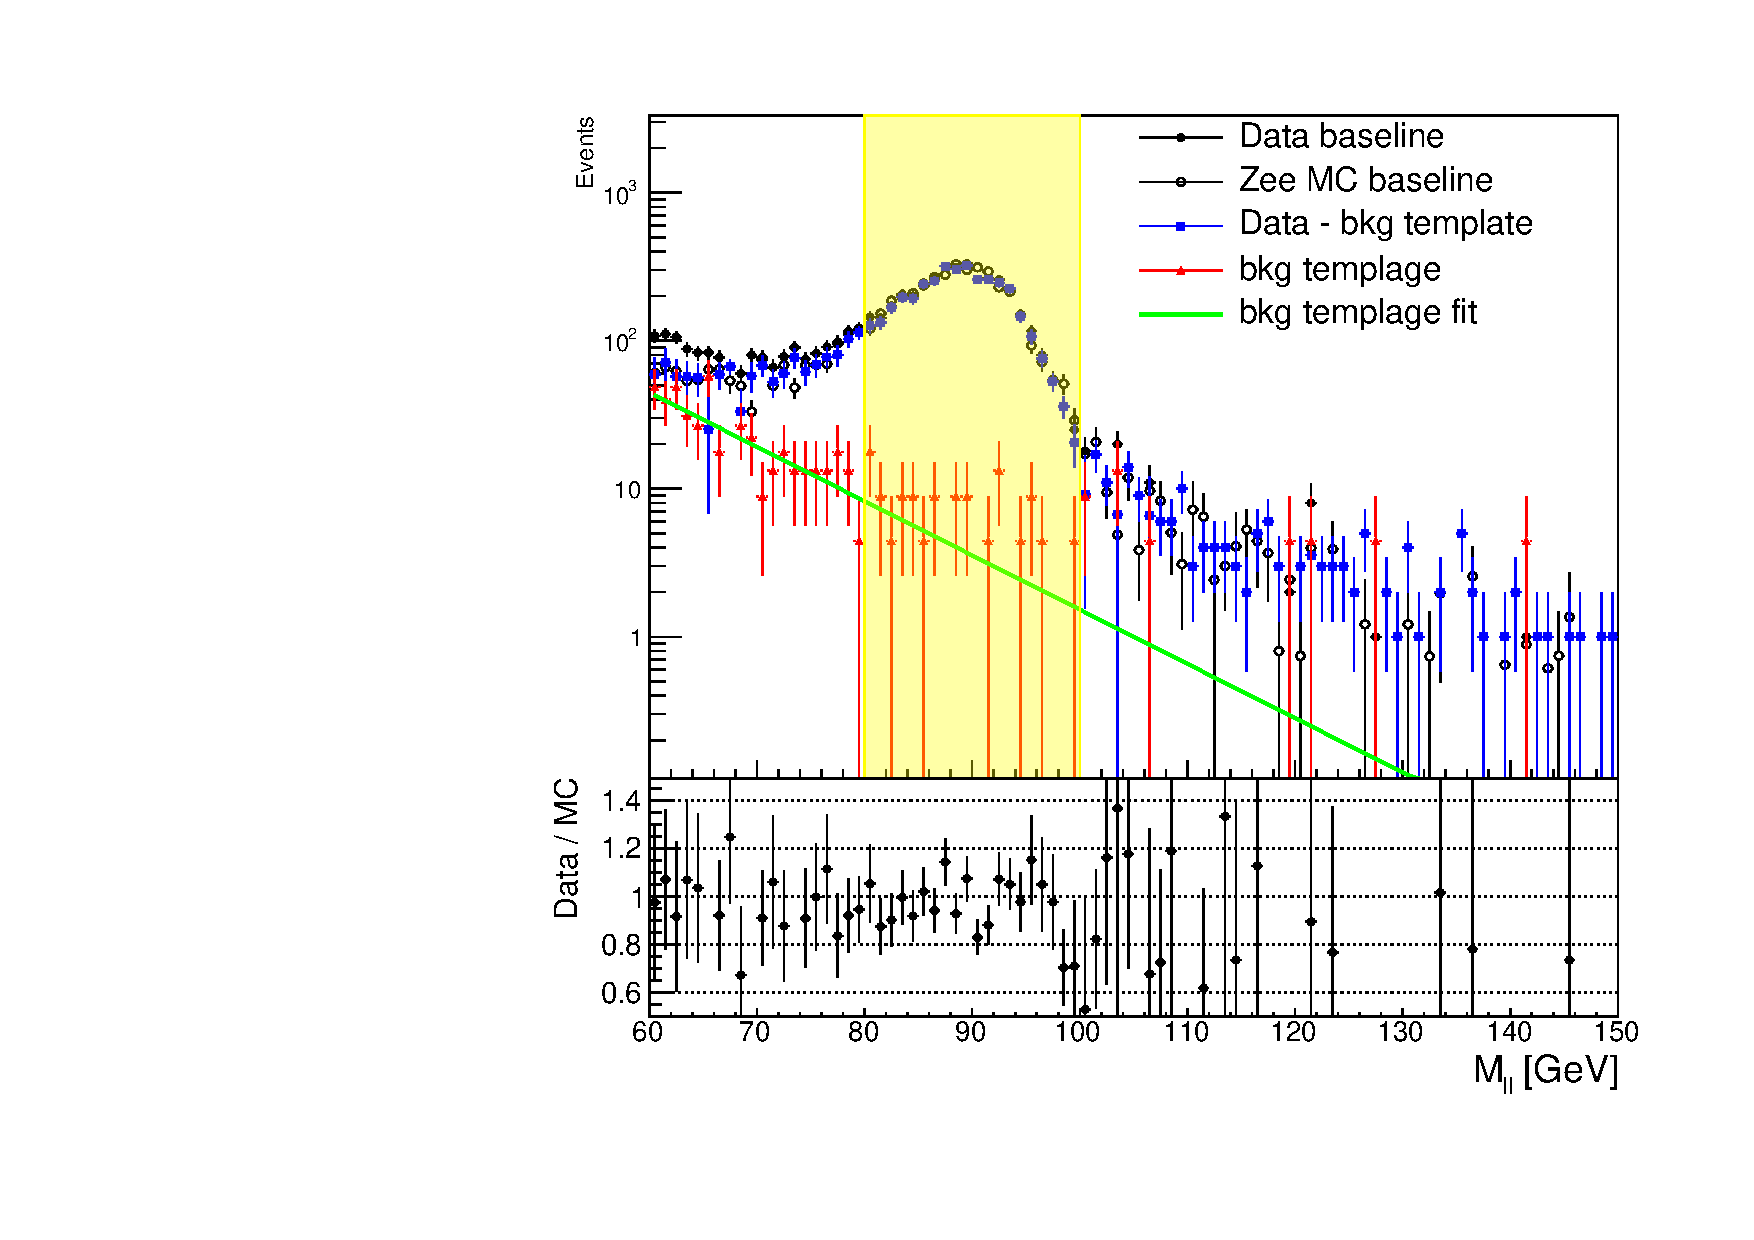
\includegraphics[scale=0.27]{bkg_subtraction_baseline_template_range_baseline_mll80_100_pt10_15_eta80_137_tag_trigger_matched.pdf}
            \caption{$10 < \pt < 15$~{\GeV}\\$0.8 < |\eta| < 1.37$}
        \end{center}
    \end{subfigure}
    \begin{subfigure}[b]{0.32\textwidth}
        \begin{center}
            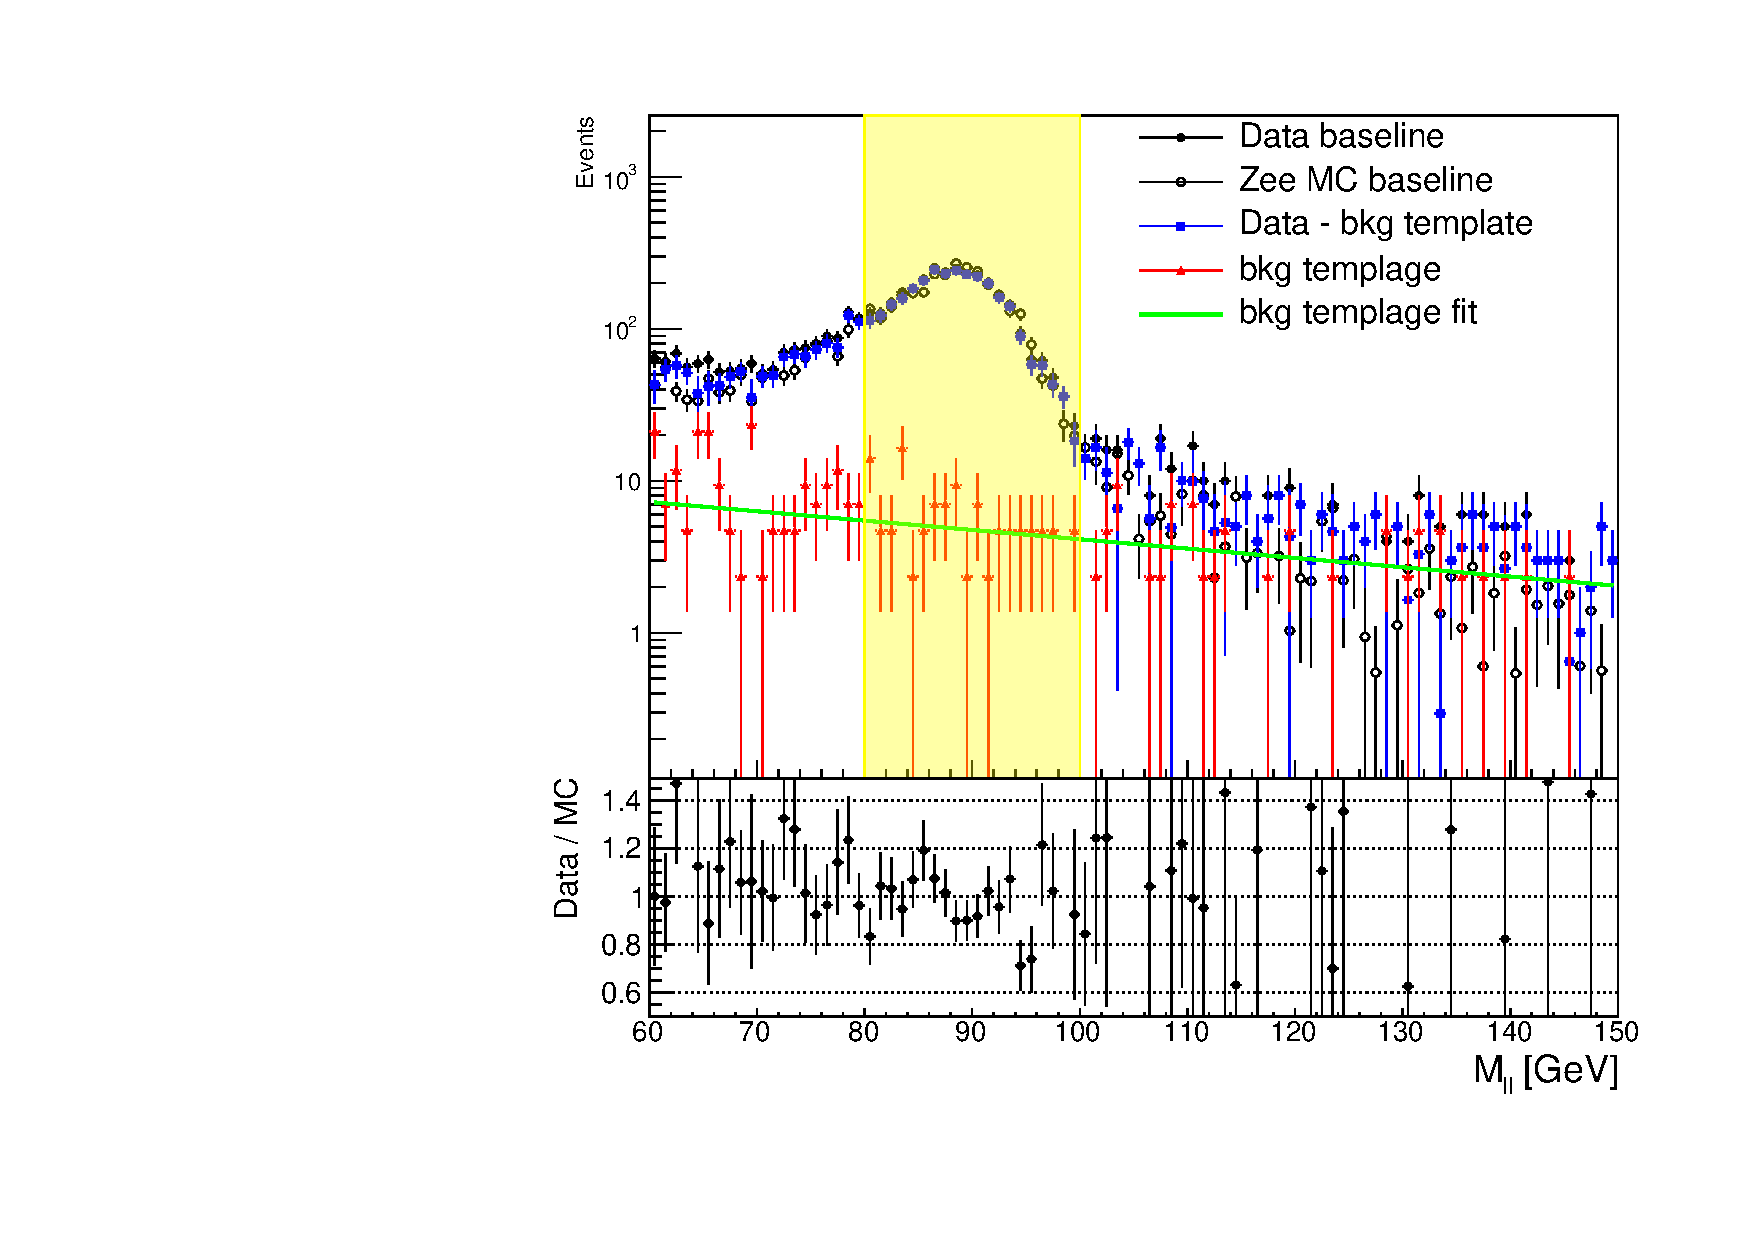
\includegraphics[scale=0.27]{bkg_subtraction_baseline_template_range_baseline_mll80_100_pt10_15_eta151_200_tag_trigger_matched.pdf}
            \caption{$10 < \pt < 15$~{\GeV}\\$1.52 < |\eta| < 2.0$}
        \end{center}
    \end{subfigure}
    \\
    \begin{subfigure}[b]{0.32\textwidth}
        \begin{center}
            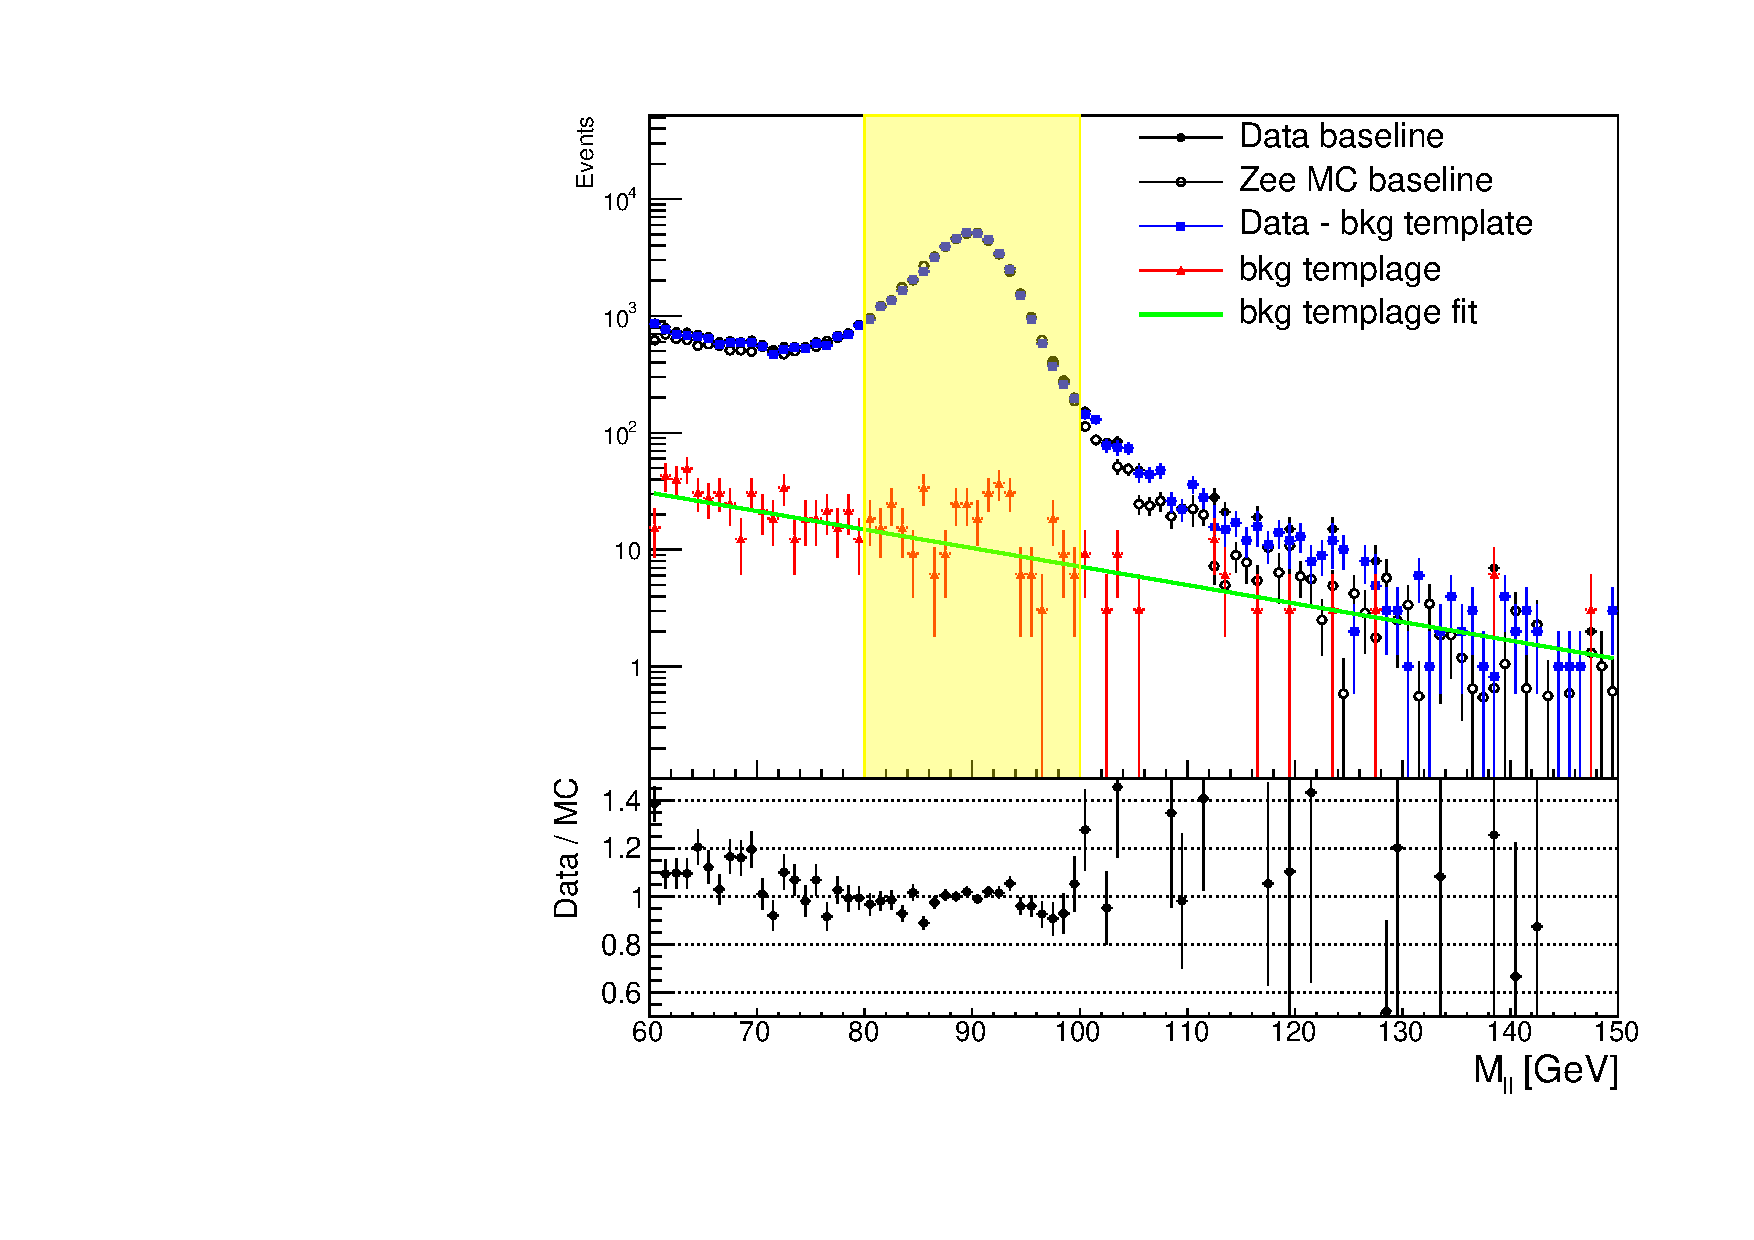
\includegraphics[scale=0.27]{bkg_subtraction_baseline_template_range_baseline_mll80_100_pt15_20_eta0_80_tag_trigger_matched.pdf}
            \caption{$15 < \pt < 20$~{\GeV}\\$0 < |\eta| < 0.8$}
        \end{center}
    \end{subfigure}
    \begin{subfigure}[b]{0.32\textwidth}
        \begin{center}
            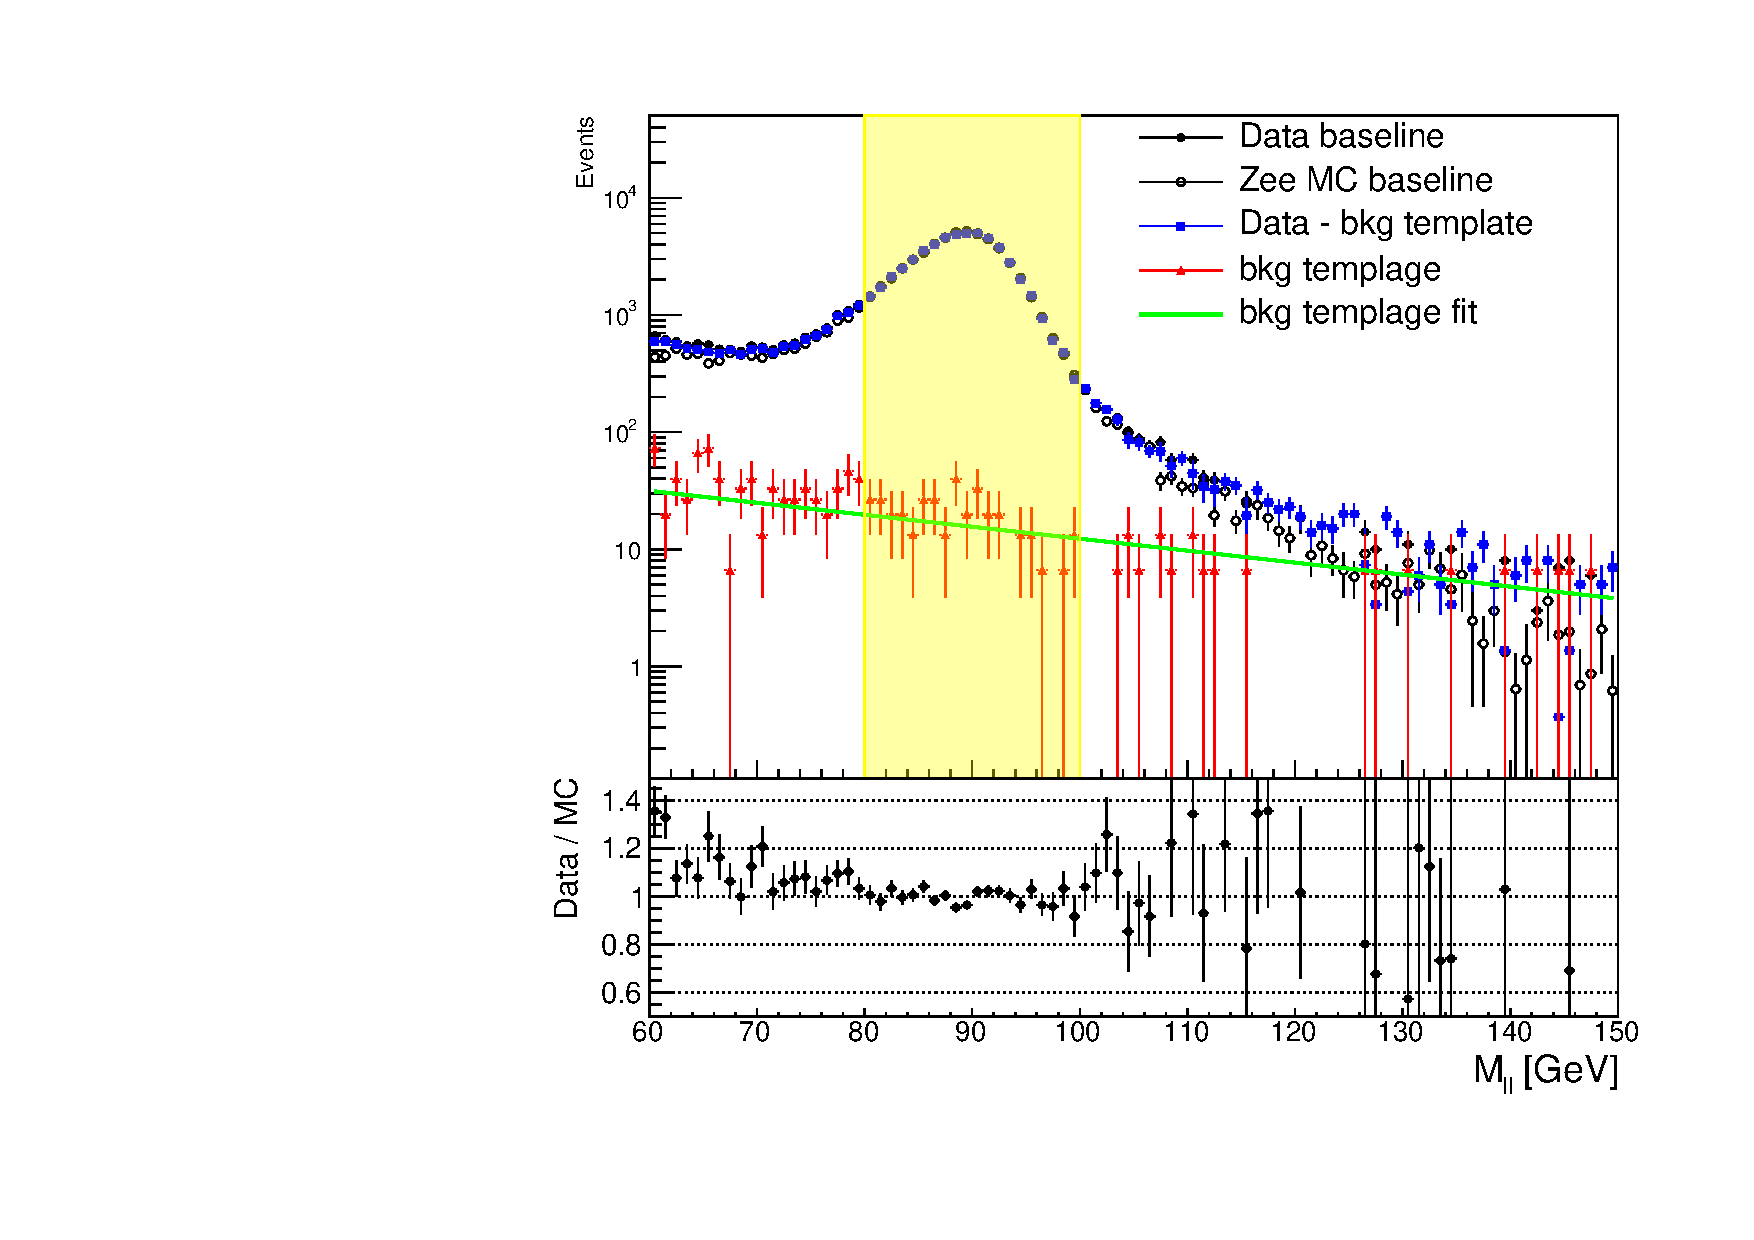
\includegraphics[scale=0.27]{bkg_subtraction_baseline_template_range_baseline_mll80_100_pt15_20_eta80_137_tag_trigger_matched.pdf}
            \caption{$15 < \pt < 20$~{\GeV}\\$0.8 < |\eta| < 1.37$}
        \end{center}
    \end{subfigure}
    \begin{subfigure}[b]{0.32\textwidth}
        \begin{center}
            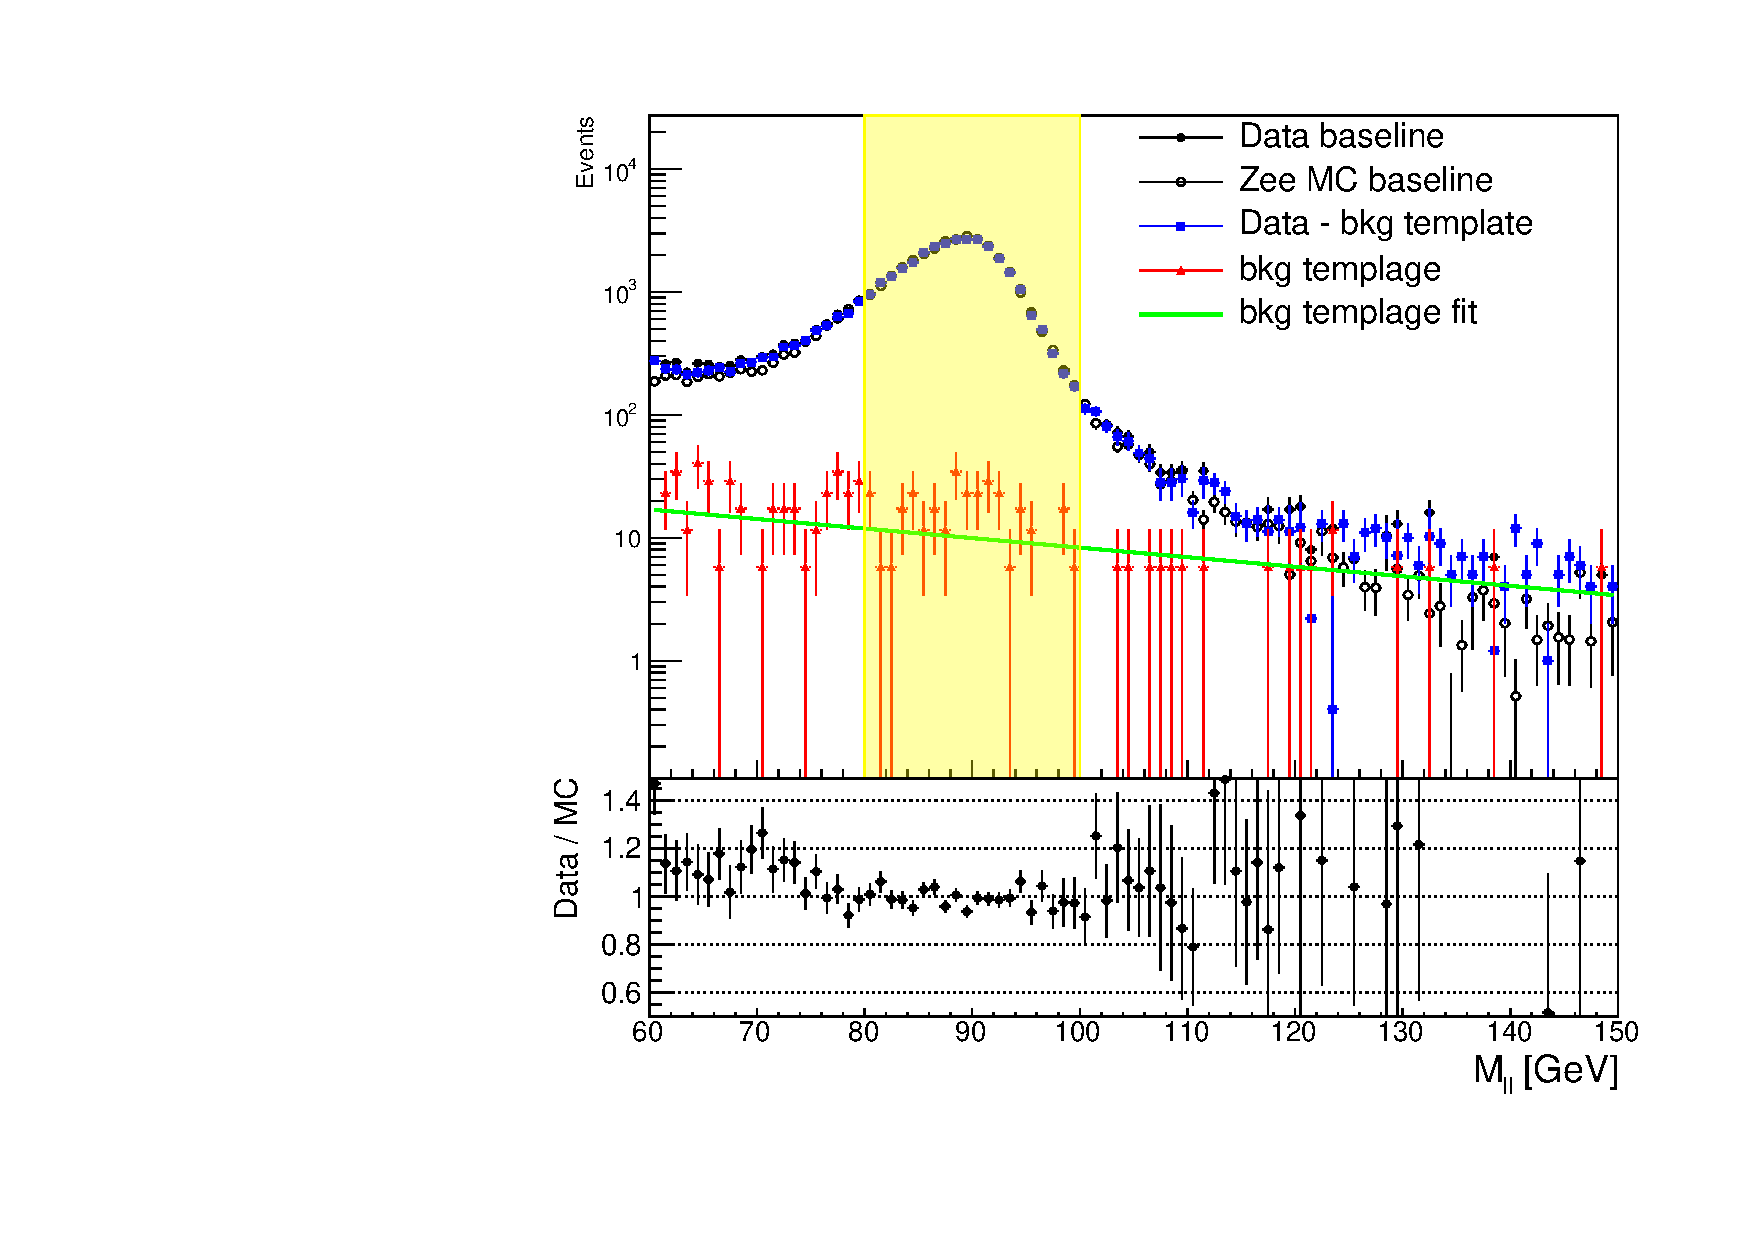
\includegraphics[scale=0.27]{bkg_subtraction_baseline_template_range_baseline_mll80_100_pt15_20_eta151_200_tag_trigger_matched.pdf}
            \caption{$15 < \pt < 20$~{\GeV}\\$1.52<|\eta|<2.0$}
        \end{center}
    \end{subfigure}
    \caption{Illustration of the background subtraction procedure.
    The full black dots and blue squares are the $m_{ee}$ distributions for data before and after performing the background subtraction, respectively.
    The $m_{ee}$ distribution for $Z \to ee$ MC, which is labeled by the open black circles, is normalized to the data after the background subtraction using a Gaussian fit of $85 < m_{ee} < 95$~{\GeV}.
    The lower panels show the data-to-MC ratio where the background subtraction has been applied on data.
    The background templates and their respective fitting results are indicated by the red triangles and green lines, respectively.
    }
    \label{fig:app_RLE_bkg_estimations}
\end{figure}
%
The data after performing the background subtraction, the MC simulation samples, the background template distributions, and the fitting results are also shown.
The simulated $m_{ee}$ distribution of $Z \to ee$ MC are normalized to the data, which background subtraction has been performed, using a Gaussian fit in $Z$ peak region $85 < m_{ee} < 95$~{\GeV}.
After performing the background subtraction, the data and MC have good agreement within the statistical uncertainties.

Then, the background contamination in the $Z$ mass region $80 < m_{ee} < 100$~{\GeV} is calculated using
%
\begin{equation}
    N_{bkg}^{80 < m_{ee} < 100~{\GeV}} = \int_{80}^{100} N_\mathrm{template} \ dm_{ee} \cdot \frac{N_{bkg}^\mathrm{tail}}{N_\mathrm{template}^\mathrm{tail}}
    \label{eq:RLE_bkg_in_80_mll_100}
\end{equation}
%
Table~\ref{tab:app_RLE_bkg_estimations} summarize the background estimations in different \pt and $|\eta|$ regions.
%
\begin{table}[htbp]
    \begin{center}
        \begin{tabular}{cccc}
            \hline
            \hline
                                  & $0 < |\eta| < 0.8$ & $0.8 < |\eta| < 1.37$ & $1.52 < |\eta| < 2.0$\\
            \hline
            $10< \pt < 15$~{\GeV} & 4.04\%             & 2.10\%                & 3.17\%\\
            $15< \pt < 20$~{\GeV} & 0.44\%             & 0.58\%                & 0.76\%\\
            \hline
            \hline
        \end{tabular}
    \end{center}
    \caption{The estimated background contamination in in different \pt and $|\eta|$ regions.
    The \pt and $|\eta|$ binnings correspond to the one used for the final measurements.}
    \label{tab:app_RLE_bkg_estimations}
\end{table}
%
The largest improvements are observed in the lowest \pt bin ($10 < \pt < 15$~{\GeV}) where a sizeable background contamination is subtracted.
The background contamination is relatively small in the second lowest \pt bin ($15 < \pt < 20$~{\GeV}) providing the evidence that high purity of prompt leptons can be obtained using $Z$ tag-and-probe method.
Table~\ref{tab:app_RLE_efficiency_before_and_after_background_subtraction} shows the real electron efficiencies before and after performing the background subtraction.

\begin{table}[htbp]
    %\begin{center}
    \resizebox{\textwidth}{!}{% <------ Don't forget this %
        \begin{tabular}{ccccc}
            \hline
            \hline
                                                    & background subtraction & $0 < |\eta| < 0.8$ & $0.8 < |\eta| < 1.37$ & $1.52 <| \eta| < 2.0$\\
            \hline
            \multirow{2}{*}{$10 < \pt < 15$~{\GeV}} & before                 & $57.4 \pm 0.9$     & $66.6 \pm 0.8$        & $53.2 \pm 0.9$\\
                                                    & after                  & $59.9 \pm 1.9$     & $68.0 \pm 1.8$        & $55.0 \pm 1.7$\\
            \hline
            \multirow{2}{*}{$15 < \pt < 20$~{\GeV}} & before                 & $64.5 \pm 0.2$     & $69.4 \pm 0.2$        & $62.0 \pm 0.3$\\
                                                    & after                  & $64.8 \pm 0.5$     & $69.8 \pm 0.5$        & $62.5 \pm 0.6$\\
            \hline
            \hline
        \end{tabular}
    }
    %\end{center}
    \caption{The real electron efficiencies before and after performing the background subtraction in different \pt and $|\eta|$ regions are shown in percentage.}
    \label{tab:app_RLE_efficiency_before_and_after_background_subtraction}
\end{table}

%%%
%%%
%%%

\section{Cut efficiencies}
\label{sec:app_RLE_cut_efficiencies}
Figure~\ref{fig:app_RLE_cut_efficiencies} shows the efficiencies associated to each signal cut with respect to baseline definitions.
%
\begin{figure}[htbp]
    \begin{subfigure}[b]{0.48\textwidth}
        \begin{center}
            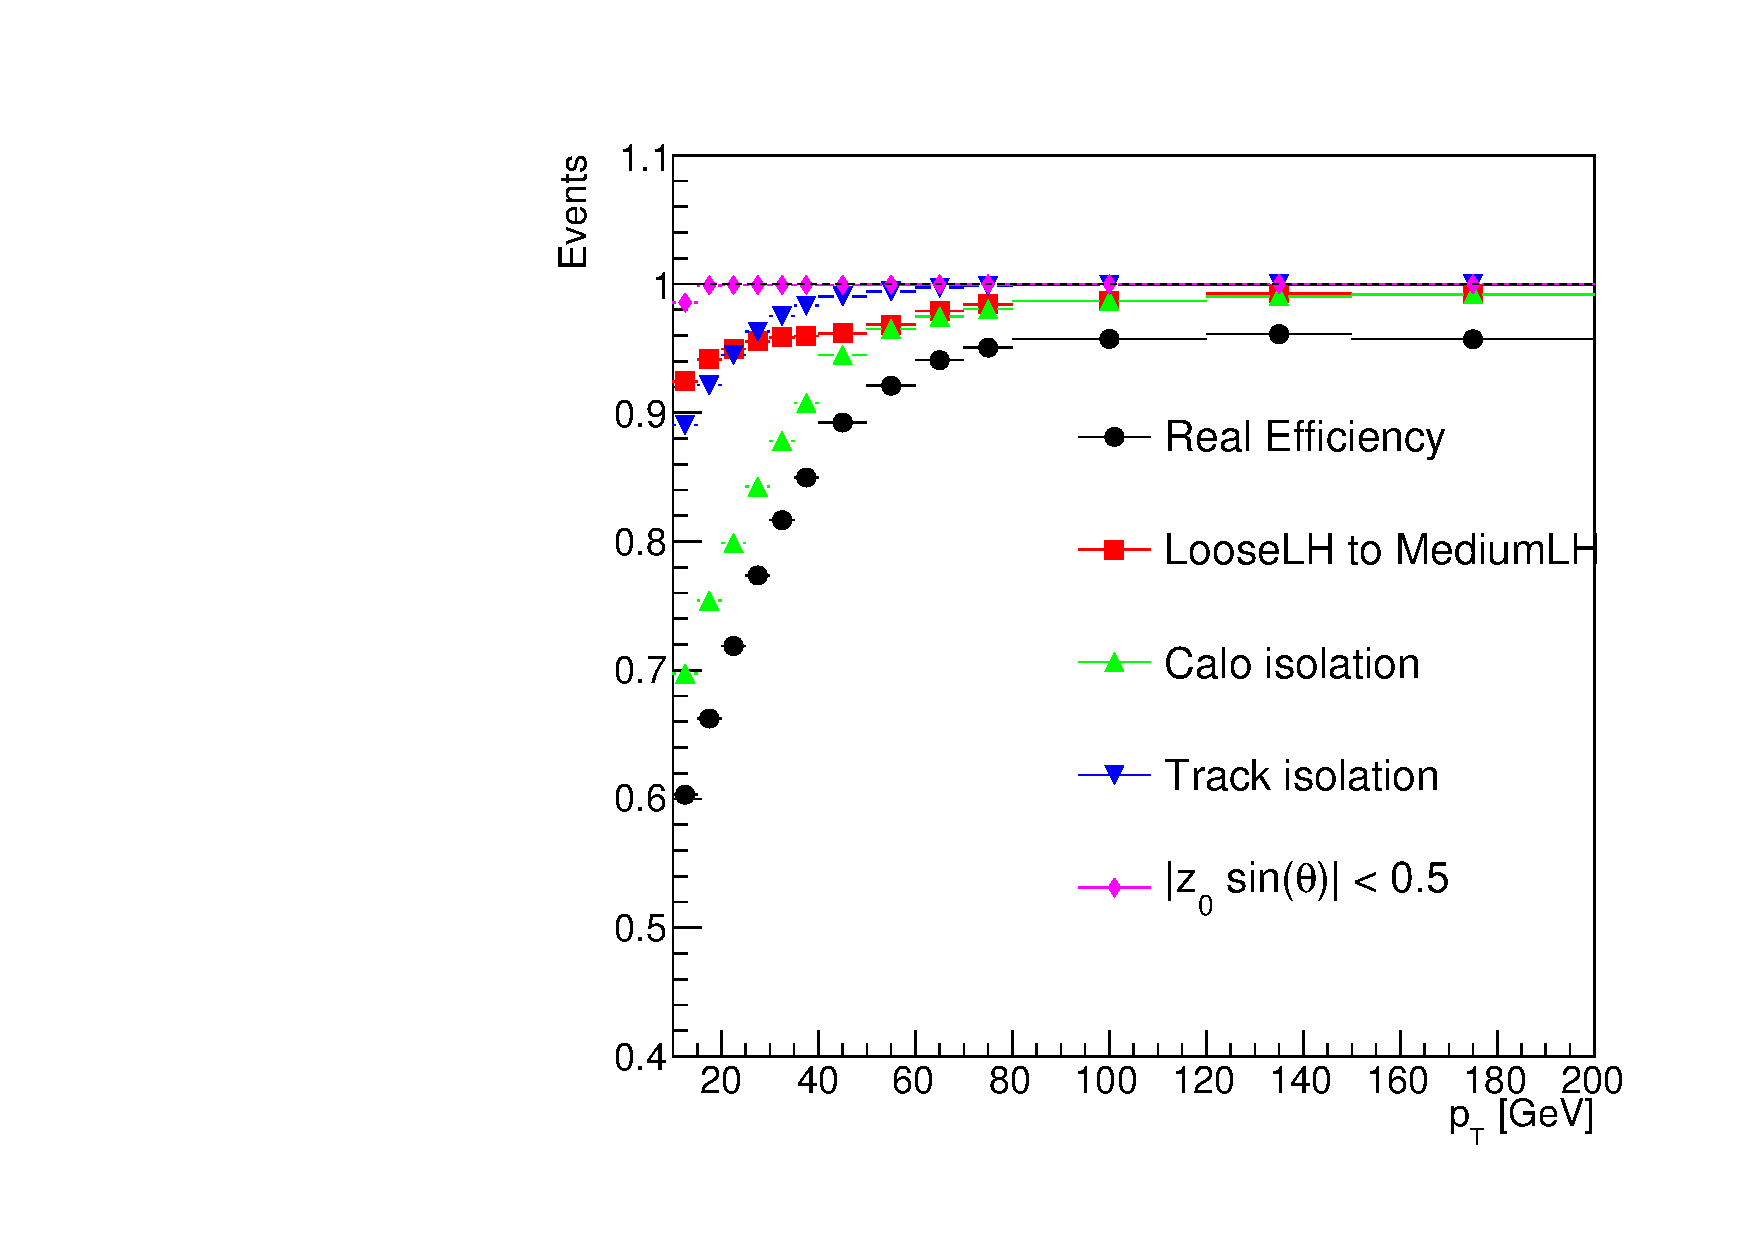
\includegraphics[scale=0.27]{cut_efficiency_electron.pdf}
            \caption{Electron}
        \end{center}
    \end{subfigure}
    \begin{subfigure}[b]{0.48\textwidth}
        \begin{center}
            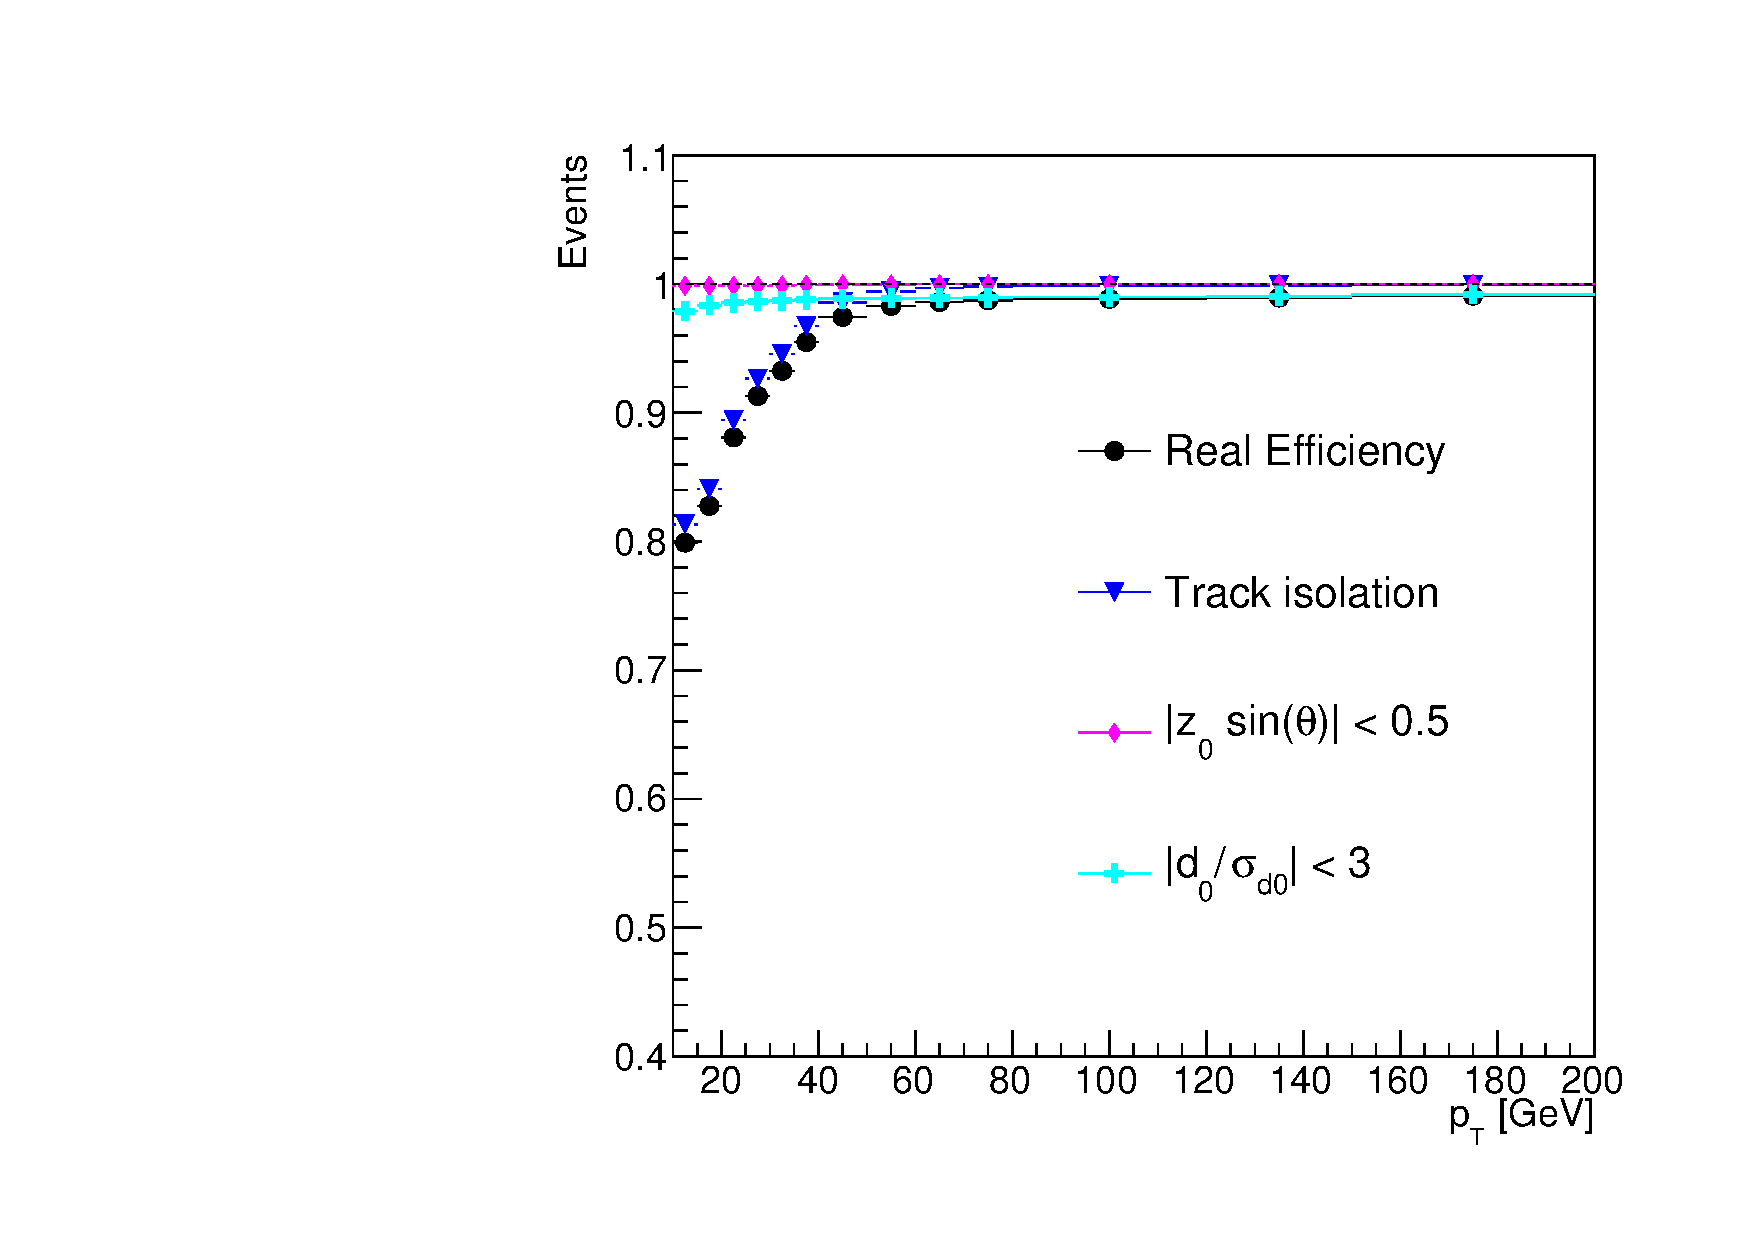
\includegraphics[scale=0.27]{cut_efficiency_muon.pdf}
            \caption{Muon}
        \end{center}
    \end{subfigure}
    \caption{Cut efficiencies of the signal electron and muon definition as a function of \pt.
    The total real electron and muon efficiencies are presented by black points. 
    The loose to medium likelihood cut efficiency is presented by red squares.
    The calorimeter and track isolation cut efficiencies are presented by green triangles and blue triangles, respectvely.
    The longitudinal and tranverse impact parameters cut efficiencies are presented by magenta diamonds and cyan crosses, respectively.}
    \label{fig:app_RLE_cut_efficiencies}
\end{figure}
%















The real lepton efficiency is defined as the ratio between the number of prompt leptons passing the signal lepton definitions and the number of prompt leptons passing the baseline lepton definitions (as presented in section~\ref{sec:objects}). Thus, it measures the efficiency of the signal lepton definition cuts with respect to the baseline ones.




The left plot in Figure~\ref{fig:RLE_cut_efficiencies} shows that the prompt electron efficiency increases from $\sim$62\% in the $10<\pt<\SI{15}{GeV}$ region to $\sim$98\% when $\pt>\SI{80}{GeV}$.
The dominant contribution to the electron efficiency losses is the calorimeter isolation.
The loose to medium likelilihood (LH) cut efficiency increases from $\sim$92\% to $\sim$96\% in the $10<\pt<\SI{30}{GeV}$ region then reaches a plateau for $30<\pt<\SI{50}{GeV}$ and increases again to $\sim$98\% when $\pt>\SI{60}{GeV}$.
The calorimeter isolation cut efficiency increases from $\sim$ 69\% in the $10<\pt<\SI{15}{GeV}$ region to $\sim$98\% when $\pt>\SI{70}{GeV}$.
The efficiency associated to the track isolation cut is $\sim$89\% for $10<\pt<\SI{15}{GeV}$ and increases up to $\sim$100\% when $\pt>\SI{60}{GeV}$.
The contribution of the longitudinal impact parameter cut to the real efficiency is $\sim$98\% for $10<\pt<\SI{15}{GeV}$ and increases up to $\sim$100\% when $\pt>\SI{15}{GeV}$.

As the same muon identification is used for the baseline and the signal definitions, the muon efficiencies are much higher than the electron ones (Figure~\ref{fig:RLE_cut_efficiencies}, right hand side).
The associated efficiencies computed using $Z\to \mu \mu$ events increase from $\sim$80\% for $10<\pt<\SI{15}{GeV}$ to $\sim$98\% when $\pt>\SI{50}{GeV}$.
The dominant contribution to the muon efficiency is the track isolation cut. The associated efficiency increases from $\sim$82\% to 98\% when $\pt>\SI{50}{GeV}$.
Another difference with the electron case is that a transverse impact parameter cut is used in the muon signal definitions while this cut is already applied at the baseline level in the electron case.
The contributions of the longitudinal and transverse impact parameter cuts on muon efficiency are very small because the cut efficiency of transverse impact parameter is $\sim$99\% and the longitudinal one is 100\%.

%%%
%%%
%%%

\subsubsection{Real lepton efficiencies}
\label{subsubsec:RLE_results}

Figure~\ref{fig:RLE_real_efficiency_total_systematics} shows the real lepton efficiencies as a function of \pt and $|\eta|$ used by the matrix method.
The three $|\eta|$ binnings used for the electron case are driven by the electromagnetic calorimeter geometry.
The background subtraction has been applied on the $10<\pt<\SI{15}{GeV}$ and $15<\pt<\SI{20}{GeV}$ for the electron case.
Because the crack region, $1.37<|\eta|<1.52$, is not considered in the analysis, this region is removed from the real electron efficiency study.
The uncertainties are the quadratic sum of the statistical uncertainties and the measurement systematic uncertainties.
The electron efficiencies in $1.52<|\eta|<2.01$ are lower than the other two $|\eta|$ regions.
This is expected as the electron identification is better in the central region of the calorimeter. 

\begin{figure}[htbp]
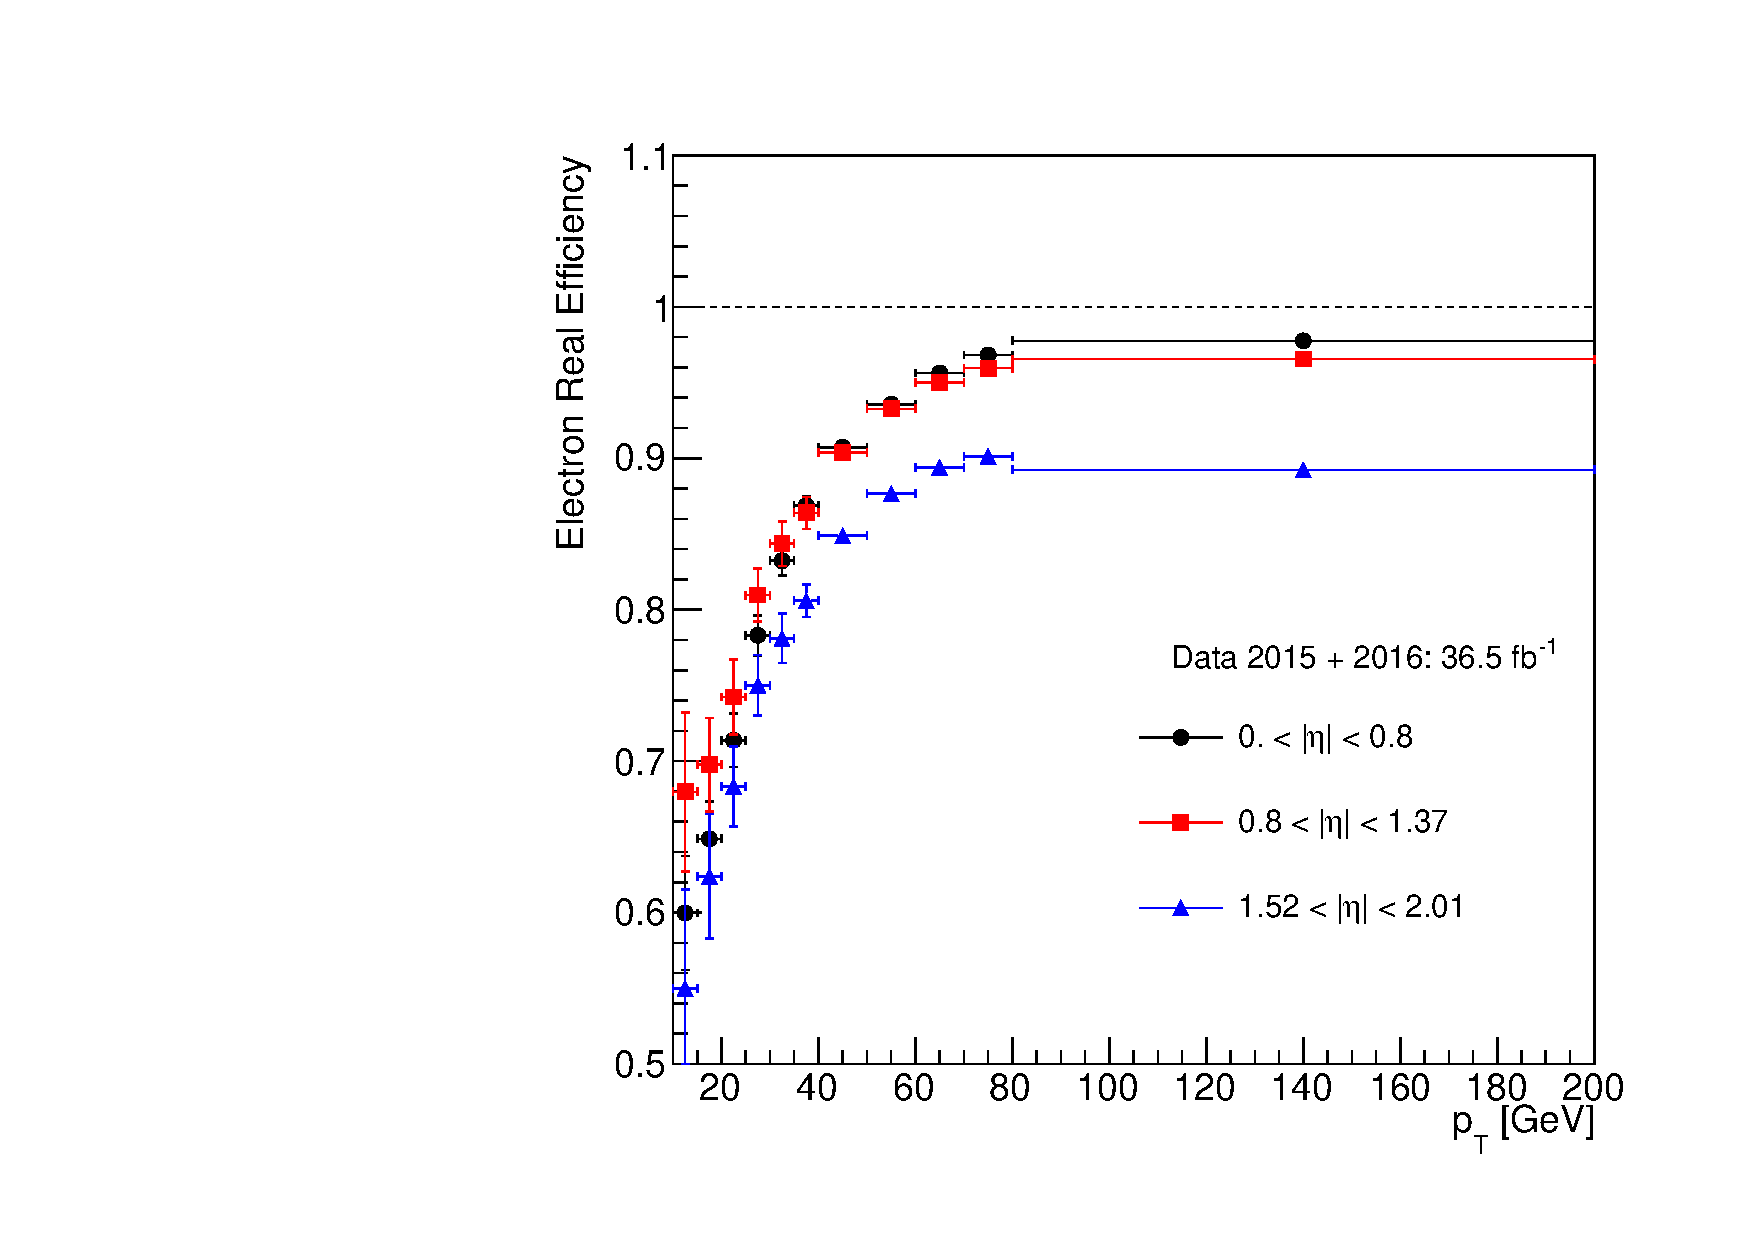
\includegraphics[width=0.48\textwidth]{real_electron_efficiency_total_systematics.pdf}
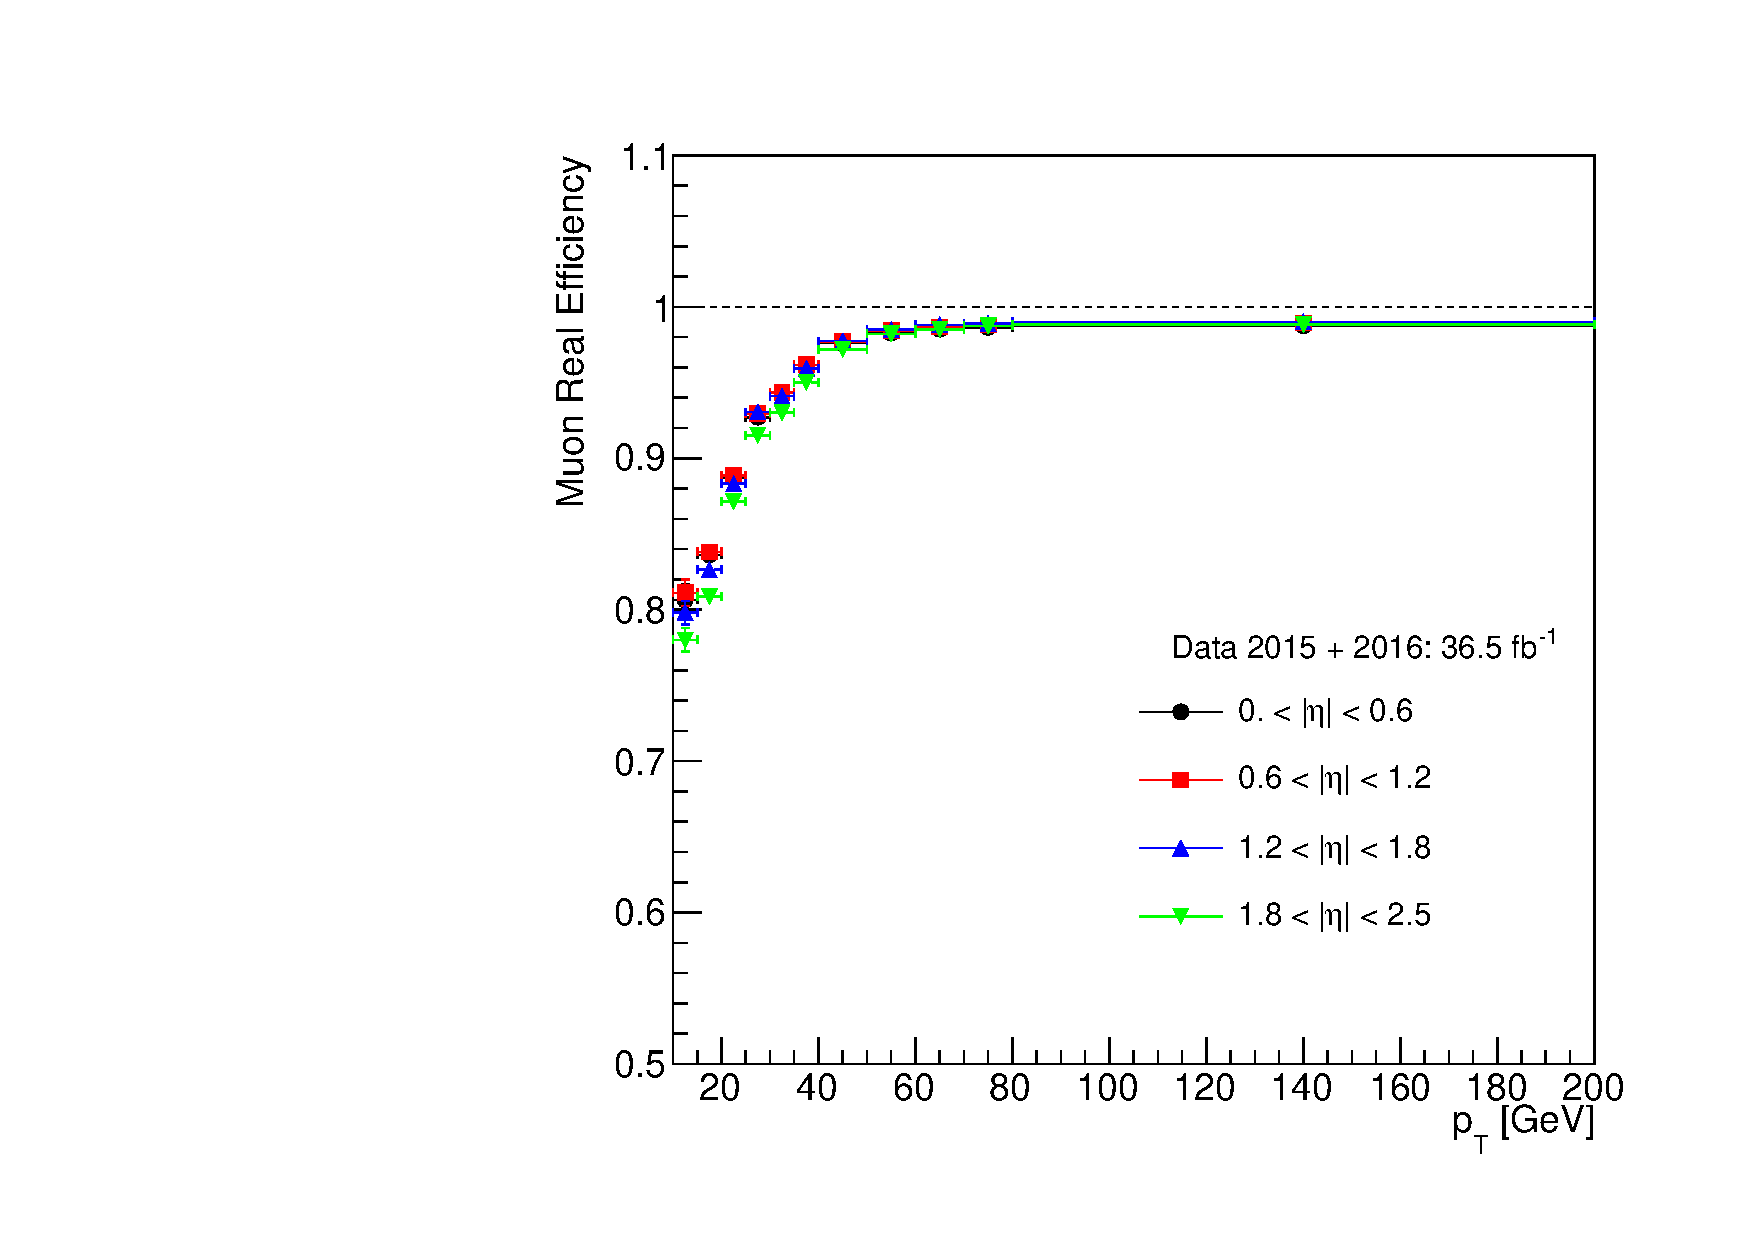
\includegraphics[width=0.48\textwidth]{real_muon_efficiency_total_systematics.pdf}
\caption{The real lepton efficiencies as a function of \pt and $|\eta|$ measured using the $Z$ tag-and-probe method.
The left plot corresponds to the real electron efficiencies in three $|\eta|$ regions and the right plot stands for the real muon efficiencies in four $|\eta|$ regions.
The $|\eta|$ binning used for the real electron efficiencies measurement corresponds to the geometry of the electromagnetic calorimeter and removing the creak region.
A homogeneous $|\eta|$ binning has been chosen for the muon case.}
\label{fig:RLE_real_efficiency_total_systematics}
\end{figure}